\documentclass{sig-alternate}

\usepackage[usenames, dvipsnames]{color}
\usepackage{times}
\usepackage{xspace}
\usepackage{textcomp}
\usepackage{wrapfig}
\usepackage{url}
\usepackage{amsmath, amssymb}
\usepackage[protrusion=true,expansion=true]{microtype}


\usepackage{alltt}
\usepackage{appendix}
\usepackage{algorithm}
\usepackage{algorithmic}

\usepackage{txfonts}
\newcommand{\Tau}{\mathcal{T}}
\newcommand{\SDedalus}{\mathcal{S}}
\newcommand{\Consts}{\mathcal{C}}
\newcommand{\Vars}{\mathcal{A}}
%\newcommand{\pos}{\protect{$_{pos}$}}
%\newcommand{\nega}{\protect{$_{neg}$}}
% RCS: Would like to use the above ones, but can't get them to work in Dedalus env.
\newcommand{\pos}{\_pos}
\newcommand{\nega}{\_neg}

\newcommand{\jmh}[1]{{\textcolor{red}{#1 -- jmh}}}
\newcommand{\paa}[1]{{\textcolor{blue}{#1 -- paa}}}
\newcommand{\rcs}[1]{{\textcolor{green}{#1 -- rcs}}}
\newcommand{\nrc}[1]{{\textcolor{magenta}{#1 -- nrc}}}
\newcommand{\wrm}[1]{{\color{BurntOrange}{#1 -- wrm}}}
\newcommand{\smallurl}[1]{{\small \url{#1}}}

\newtheorem{example}{Example}
\newdef{definition}{Definition}
\newtheorem{lemma}{Lemma}
\newtheorem{observation}{Observation}

%\def\slang{synchronous Dedalus\xspace}
\def\lang{\textsc{Dedalus}\xspace}
\def\slang{\textsc{Dedalus\ensuremath{_{{0}}}}\xspace}
%\def\synclang{{Dedalus\ensuremath{_{\large 0}}}\xspace}
\newcommand{\naive}      {na\"{\i}ve\xspace}
\newcommand{\Naive}      {Na\"{\i}ve\xspace}
%dedalus environment for code

\newenvironment{Dedalus}{
\vspace{0.5em}\begin{minipage}{0.95\textwidth}%\linespread{1.3}
\begin{alltt}\fontsize{9pt}{9pt}\selectfont}
{\end{alltt}\end{minipage}\vspace{0.5em}}

\newcommand{\dedalus}[1]{\texttt{\fontsize{9pt}{9pt}\selectfont #1}}


\begin{document}

\conferenceinfo{ACM PODS}{'10 Indianapolis, IN, USA}
\title{{\huge{\bf\lang}}:
Datalog in Time and Space} 
%%Format\titlenote{(Produces the permission block, copyright information and page numbering). For use with ACM\_PROC\_ARTICLE-SP.CLS V2.6SP. Supported by ACM.}}
%
% You need the command \numberofauthors to handle the "boxing"
% and alignment of the authors under the title, and to add
% a section for authors number 4 through n.

\numberofauthors{6}

\author{
%
Peter Alvaro$^\ast$ \quad William R. Marczak$^\ast$ \quad Neil
Conway$^\ast$  \\
Joseph M. Hellerstein$^\ast$ \quad 
David Maier$^\dagger$ \quad Russell Sears$^\ast$ 
\\\\
%
\fontsize{10}{10}\selectfont\itshape 
%\vspace{0.05in}
$^\ast$University of California, Berkeley \quad $^\dagger$Portland State
University\\\\ \fontsize{9}{9}\selectfont\ttfamily\upshape
%
\{palvaro,wrm,nrc,hellerstein,sears\}@cs.berkeley.edu \quad maier@cs.pdx.edu
%
}

\toappear{}

\maketitle

\begin{abstract} 
%
Recent research has explored using Datalog-based
languages to express a distributed system as a set of logical
invariants~\cite{boom-techr,loo-sigmod06}.  Two properties of distributed
systems proved difficult to model in Datalog.  First, the state of any such system
evolves with its execution.  Second, deductions in these systems may be
arbitrarily delayed, dropped, or reordered by the unreliable network links
they must traverse.  Previous efforts addressed the former by extending
Datalog to include updates, key constraints, persistence and events, and
the latter by assuming ordered and reliable delivery while ignoring delay.
These details have a semantics outside Datalog, which increases the complexity of
the language or its interpretation, and forces programmers to
think operationally.  We argue that the missing component from these previous
languages is a notion of {\em time}.

In this paper we present {\bf \lang}, a
foundation language for programming and reasoning about distributed systems.
\lang reduces to a subset of Datalog~\cite{ullmanbook} with negation, aggregate
functions, successor and choice, and admits an explicit representation of time into the
logic language.  
We show that \lang provides a declarative foundation for the two signature features of 
distributed systems: mutable state, and asynchronous processing and communication.
Given these two features, we address three important properties of programs in 
a domain-specific manner: a notion of {\em safety} appropriate to non-terminating computations, 
{\em stratified} monotonic reasoning with negation over time, and efficient evaluation
over time via a simple execution strategy.  We also provide conservative syntactic checks
for our temporal notions of safety and stratification.  Our experience implementing 
full-featured systems in variants of Datalog suggests that \lang is well-suited to the specification of
rich distributed services and protocols, and provides both cleaner semantics and richer tests of correctness.
\end{abstract}

\section{Introduction} 
\label{sec:intro} 
Although distributed programming has become an essential and commonplace task,
it remains very challenging for most developers to write correct distributed
programs. The inherent difficulties of distributed computing---concurrency,
asynchrony, and partial failure---are exacerbated by the scale at which modern
distributed systems operate.

% remind reviewers that it's a database problem. can remove if accepted! 
Much of the discussion about distributed programming today revolves around data
management systems, and the tradeoffs between transactions and loose
consistency. Programmers using distributed transactions are relieved of
consistency concerns but often face significant performance and operational
challenges~\cite{Birman2009}. By contrast, programmers who use loosely
consistent systems can expect more predictable and low-latency performance, but
must reason explicitly about program correctness over inconsistent distributed
state.

In recent years there has been increased interest in techniques to help
programmers achieve correct program behavior without requiring strongly
consistent storage. This idea has been explored in two different frameworks,
\emph{Convergent Objects} and \emph{Monotonic Logic}.

\vspace{0.5em}\noindent
\textbf{Convergent Objects}: In this approach, a programmer writes encapsulated
object classes whose public methods guarantee certain properties regarding
message reordering and/or retry. For example, Statebox is an open-source library
that merges conflicting updates to data items in a key-value store; the user of
the library need only register commutative, idempotent merge
functions~\cite{statebox}. This approach has roots in research in
databases~\cite{Farrag1989,Garcia-Molina1983,Helland2009} and
groupware~\cite{Ellis1989,Sun1998}.  Shapiro et al.\ recently proposed a model
for these approaches called \emph{Conflict-Free Replicated Data Types} (CRDTs),
which formalizes these ideas in an algebraic framework~\cite{Shapiro2011b}.

The main problem with the CRDT approach is that its guarantees of correctness
are limited to an individual replicated data value, not to application logic in
general. For example, consider a distributed algorithmic trading service that
uses a CRDT to represent a mutable set \texttt{Portfolio}. Suppose one server
$M$ reads a local version of the set containing an element \texttt{BNNA} and
constructs an expected portfolio value $v = f(\mbox{\texttt{Portfolio}})$
derived from that version. Concurrently, \texttt{BNNA} is removed from the local
version of \texttt{Portfolio} at another server $N$. The CRDT can ensure that
$M$ and $N$ will eventually agree that \texttt{BNNA} is absent from the set, but
the application state at $M$ and $N$ may remain inconsistent unless the value
$v$ at $M$ is updated to reflect the removal of \texttt{BNNA}. Although the CRDT
maintains its own invariants, the programmer still bears the burden of ensuring
the consistency semantics of the entire program.

\vspace{0.5em} \noindent
\textbf{Monotonic Logic}: In recent work, we observed that the database theory
literature on non-monotonic logic provides a promising starting point for
reasoning about distributed consistency. Intuitively, a \emph{monotonic} program
computes more information over time---it never ``retracts'' an earlier
conclusion in the face of new information. We proposed the CALM
theorem~\cite{Hellerstein2010}, which established that all monotonic programs
are eventually consistent~\cite{Ameloot2011,dedalus-pods12-tr}. Monotonicity of
a Datalog-style program is straightforward to determine conservatively from
syntax, so the CALM theorem provides the basis for a simple analysis technique
for verifying the consistency of distributed programs~\cite{Alvaro2011}. We
realized the CALM analysis as part of Bloom, a Datalog-based DSL for distributed
programming~\cite{bloom}.

The original formulation of Bloom and CALM only validated consistency for programs that compute sets of facts that grow over time (``set monotonicity''); that is, ``growth'' is defined according to set containment. As a practical matter, this is overly conservative: several common distributed programming idioms that are monotonic do not satisfy syntactic monotonicity tests for Datalog. In particular, threshold tests over monotonic aggregate values (e.g., ``$\mathrm{max}(S) > k$'') and upward-moving mutable counters are both considered to be non-monotonic by the original CALM analysis.  As a result, the initial Bloom prototype advises the programmer to guard those constructs with strong consistency methods like Paxos~\cite{Lamport1998} or Two-Phase Commit. 

\subsection{A Hybrid Approach}
% The strengths and weaknesses of these two approaches appear complementary. CRDTs provide synchronization-free consistent objects, but cannot guarantee whole-program consistency. Bloom's CALM analysis guarantees whole-program consistency but is unable to verify a number of natural coordination-free mechanisms.
In this paper, we extend our previous work to accommodate the ideas underlying CRDTs. Instead of only allowing growth according to the set containment
partial order, we allow any user-defined partial order to be used.  
We do this by providing \emph{join semi-lattices} as a programming construct.
We give a
formal definition of this construct below, but the intuition is that the programmer provides a commutative, idempotent merge function (``least upper bound'')
that takes two input values and produces an output value that is not smaller
than either of the input values (according to the user's partial order). This
generalizes Bloom (and traditional Datalog), which assumes a fixed merge
function (set union) and partial order (set containment).
% Relate user-defined merge functions to merge functions in other contexts?
% (e.g., key-value store, COPS, Piccolo)

% Explain how lattices generalize monotonic datalog
It is attractive to incorporate join semi-lattices into logic programming,  but doing so raises challenges in language design, consistency analysis and efficient execution.  In this paper, we make the following contributions:
\begin{enumerate}
% \item
%   We present \baselang, a variant of Datalog that is defined over lattices. We
%   define a model-theoretic semantics for \baselang, and show that \baselang
%   generalizes Datalog.

\item
  We introduce \lang, an extension of Bloom that supports lattices. We detail
  the builtin lattice types provided by \lang and show how developers can
  define new lattices.
  
\item 
  We provide interfaces for consistency-preserving mappings across lattices via
  \emph{morphisms} and \emph{monotonic functions}.  This is critical for \lang
  and forms a useful extension to the CRDT framework as well.

\item 
  We generalize the CALM analysis to programs that contain both lattices and
  set-oriented collections, and show how lattices can be used to prove the
  confluence of several common distributed design patterns that were regarded as
  non-monotonic in Bloom. % XXX: revisit this

\item
  For efficient execution, we show how to extend the standard Datalog semi-naive
  evaluation scheme~\cite{Balbin1987} to support both lattices and traditional
  database relations. We also describe how an existing Datalog engine can be
  extended to support lattices with relatively minor changes.

\item
  Finally, we demonstrate the usefulness of lattices with two case studies.
  First we revisit the simple e-commerce scenario presented in Alvaro et al., in
  which clients interact with a replicated shopping cart
  service~\cite{Alvaro2011}. We show how \lang can be used to make the
  ``checkout'' operation monotonic, despite the fact that it requires
  aggregating over a distributed data set.

  Second, we use \lang to implement vector clocks and causal delivery, two
  standard building blocks for distributed programming. We show how both
  algorithms can be realized as monotonic \lang programs that are concise and
  readable.
\end{enumerate}

\section{\large \bf \lang}
\label{sec:foundation}

To arrive at a formal semantics for distributed programs, we present the \lang~\cite{dedalus} language, which formally captures the intuitive notion of logic programs being executed asynchronously across the nodes of a distributed system.
In designing \lang, we extended the well-understood Datalog language with temporal constructs that allowed
us to model time-varying state and channel reordering and delay.  As we shall see, both extensions are made
possible by admitting a representation of logical time into the program schema, allowing the consequences of
deductions to hold ``at a different time'' than their antecedents.  By narrowly constraining such temporal 
deductions, we argue that \lang captures salient features of systems that communicate over unreliable networks and mutate state over time.

%\todo{Get rid of ``stable model semantics''}
We begin this section by reviewing the syntax of \lang that was first presented in~\cite{dedalus}. We then move on from that beginning by providing a model-theoretic semantics for \lang.  We note that the stable model semantics may be
used to assign meanings to \lang programs that capture the mutation of state over logical time, much as an execution trace \jmh{do you want to cite somebody theoretical for a definition of a trace in imperative-land?  E.g. I/O Automata ``executions''?} captures the behavior of a
typical imperative distributed program over time.  
This interpretation presents certain obstacles:
even if a \lang program has a deterministic final state, channel nondeterminism may induce an infinite number of stable models, each corresponding to a superficially different evolution toward that state over logical time.  To project away the (potentially infinite) variety of these distinctions, we present the {\em ultimate model} semantics, an abstraction that associates a program with a finite model of 
its ``eventual'' execution state.  Even with this simplification, some programs may have more than one ultimate model.  We conclude by showing a natural correspondence between the multiple ultimate models and sensitivities of the specification to the main non-determinism inherent in distributed systems: message delays and reordering.  

\jmh{I shortened the end of the above as I think you were skidding into deeper water than you want to explain here in an intro.}

\jmh{PS: Should we make an argument that the ultimate models cover all possible message orderings?  Or all ``interesting'' (non-commuting) permutations of messages?}

\subsection{Syntax}

\subsubsection{Preliminary Definitions}

%\todo{Thread a running example through the paper}
%\todo{ensure ``relation'' vs ``relation name'' usage is consistent}
\todo{define ``relation'', ``maps''?}
\todo{Put in examples of notation close to where the notation is introduced -Dave Maier}

We assume a finite universe $\univ$ of values.

A {\em relation schema} $(\dedalus{r},n)$ is a pair consisting of a relation name $\dedalus{r}$ and its arity $n$.
A {\em database schema} $\schema$ is a finite set of relation schemas.
%\nrc{Confusing: relation schema is a singleton, but ``schema'' is a set of relation schemas?} 
%I'm changing ``schema'' to ``database schema''.  A google search for [``relational schema'' ``database schema''] reveals this to be at least somewhat standard.

A {\em fact} over a relation schema $(\dedalus{r}, n)$ is a pair consisting of
the relation name \dedalus{r} and an $n$-tuple $(c_1,\ldots,c_n)$, where each
$c_i \in \univ$.  We denote a fact with relation name \dedalus{r} by
\dedalus{r(c\sub{1}, \ldots, c\sub{n})}.  As in~\cite{immerman-ptime}, we assume
the existence of an order: every database schema contains the relation schema
$(\dedalus{<},2)$.\footnote{We will often write \dedalus{<} in infix notation.} 
A {\em relation instance} for relation schema $(\dedalus{r},n)$ is a finite set of facts for
$(\dedalus{r},n)$.  A {\em database instance} maps each relation schema $(\dedalus{r},n) \ne
(\dedalus{<},2)$ to a relation instance for $(\dedalus{r},n)$, and maps $(\dedalus{<},2)$ to a
finite set of \dedalus{<} facts that encode a total ordering over $\univ$.

A {\em rule} over a database schema $\schema$ is a clause of the form:

\begin{Drules}
  \drule{p(\od{W})}
        {b\sub{1}(\od{X\sub{1}}), \ldots, b\sub{l}(\od{X\sub{l}}), !c\sub{1}(\od{Y\sub{1}}), \ldots, !c\sub{m}(\od{Y\sub{m}})}
\end{Drules}

\noindent where \dedalus{p}, \dedalus{b\sub{1}}, \ldots, \dedalus{b\sub{l}},
\dedalus{c\sub{1}}, \ldots, \dedalus{c\sub{m}} are relations in $\schema$, and \od{W},
\od{X\sub{i}} and \od{Y\sub{j}} denote a tuple (of the appropriate arity)
consisting of constants from $\univ$ or variable symbols.  The {\em atom} to the
left of the $\leftarrow$ is called the {\em head} of the rule, and the
conjunction of atoms to the right is called the rule's {\em body}.
%\jmh{Following on to the question above about \dedalus{<}, shouldn't we use
%  obligatory boilerplate about Horn clauses and finite Herbrand universes?}
The relation name in the rule head may not be \dedalus{<}. Furthermore, if
\dedalus{b\sub{i}} (resp.\ \dedalus{c\sub{i}}) is \dedalus{<}, then any variable
that appears in \dedalus{\od{X\sub{i}}} (resp.\ \dedalus{\od{Y\sub{i}}}) must
also appear in \dedalus{\od{X\sub{j}}} for some $b_j \neq \dedalus{<}$. That is,
variable symbols that appear in a \dedalus{<} atom must also appear in a
non-negated atom that is not \dedalus{<}.

\subsubsection{Safety}
\lang maintains the usual Datalog safety restrictions: any variable symbol
\dedalus{V} that appears in \od{Y\sub{i}} for some $1 \leq i \leq m$ must also
appear in \od{X\sub{j}} for some $1 \leq j \leq n$, but only if \dedalus{V}
appears in \od{W} or \dedalus{V} appears in \od{Y\sub{k}} for some $k \neq
i$---i.e., variable symbols that only appear in a single negated atom and do not
appear in the head need not also appear in a positive atom~\cite{ullmanbook}.
Also, any variable symbol that appears in \od{W} must appear in some
\dedalus{\od{X\sub{1}}, \ldots, \od{X\sub{l}}}.

\subsubsection{Spatial and Temporal Extensions}

Given a database schema $\schema$, we use $\sschema$ to denote the extension of $\schema$
obtained as follows. For each relation schema $(\dedalus{r}, n) \in (\schema-\{\dedalus{<}\}$), we include a relation schema $(\dedalus{r}, n+1)$ in $\sschema$. The
additional column being added to each relation schema is called a {\em location specifier}. By convention, the
location specifier is the first column of every relation in $\sschema$.
Additionally, $\sschema$ includes $\dedalus{<}$, and a relation schema $(\dedalus{node},1)$.
We call $\sschema$ a {\em spatial schema}.

A {\em spatial fact} over a relation schema of arity $n$ is a pair consisting of the relation name and an $(n+1)$-tuple $(d,c_1,\ldots,c_n)$ where each $c_i \in \univ$ and $\dedalus{node}(l)$.  A {\em spatial database instance} is defined similarly to a database instance.

Given a database schema $\schema$, we use $\stschema$ to denote the extension of
$\schema$ obtained by adding two additional columns to each relation schema in ($\schema - \{\dedalus{<}\}$) and adding four additional relation schemas to $\schema$. 
The first additional column is a location specifier, the second is a {\em timestamp}.  By convention, the location specifier is the first column of every relation in $\stschema$ and the timestamp is the second.  
The additional relation schemas we add are: $(\dedalus{node},1)$,
$(\dedalus{time},1)$, $(\dedalus{succ},2)$, and $(\dedalus{time_lt},2)$.
We call $\stschema$ a {\em spatio-temporal} schema.

A {\em spatio-temporal fact} over a relation schema of arity $n$ is a pair consisting of the relation name and an $n+2$-tuple $(d,t,c_1,\ldots,c_n)$ where each $c_i \in \univ$, \dedalus{node(l)}, and \dedalus{time(t)}.  A {\em spatio-temporal database instance} is defined similarly to a database instance, \dedalus{time(t)} for all $\dedalus{t} \in \mathbb{N}$, \dedalus{succ(x,y)} for all $y = x + 1$, and \dedalus{time_lt(x,y)} for all $x < y$.

We will use the notation \dedalus{f@t} to mean the spatio-temporal fact obtained from the spatial fact \dedalus{f} by adding a timestamp column with the constant \dedalus{t}.

A {\em spatio-temporal rule} over a spatio-temporal schema $\stschema$ is a rule of one of the following three forms:

A {\em deductive} rule:

\begin{Drules}
  \drule{p(L,T,\od{W})}
        {b\sub{1}(L,T,\od{X\sub{1}}), \ldots, b\sub{l}(L,T,\od{X\sub{l}}), !c\sub{1}(L,T,\od{Y\sub{1}}), \ldots, !c\sub{m}(L,T,\od{Y\sub{m}}), node(L), time(T)}
\end{Drules}

An {\em inductive} rule:

\begin{Drules}
  \drule{p(L,S,\od{W})}
        {b\sub{1}(L,T,\od{X\sub{1}}), \ldots, b\sub{l}(L,T,\od{X\sub{l}}), !c\sub{1}(L,T,\od{Y\sub{1}}), \ldots, !c\sub{m}(L,T,\od{Y\sub{m}}), node(L), time(T), succ(T,S)}
\end{Drules}

An {\em asynchronous} rule:

\begin{Drules}
  \drule{p(D,S,\od{W})}
        {b\sub{1}(L,T,\od{X\sub{1}}), \ldots, b\sub{l}(L,T,\od{X\sub{l}}),
          !c\sub{1}(L,T,\od{Y\sub{1}}), \ldots, !c\sub{m}(L,T,\od{Y\sub{m}}),
          node(L), time(T), time(S), time_lt(T,S), choice((L, T, \od{B}),(S)), node(D)}
\end{Drules}

The latter two kinds of rules are collectively called {\em temporal} rules.

In the above rules, \od{B} is a tuple that contains all of the distinct variable
symbols in \od{X\sub{1}}, \ldots, \od{X\sub{l}}, \od{Y\sub{1}}, \ldots,
\od{Y\sub{m}}.  The variable symbols \dedalus{D} and \dedalus{L} may appear in
any of \dedalus{\od{W}, \od{X\sub{1}}, \ldots, \od{X\sub{l}}, \od{Y\sub{1}},
  \ldots, \od{Y\sub{m}}}, whereas \dedalus{T} and \dedalus{S} may not.
Head relation name \dedalus{p} may not be \dedalus{time}, \dedalus{succ}, or \dedalus{node}.
\dedalus{b\sub{1}, \ldots, b\sub{l}, c\sub{1}, \ldots, c\sub{m}} may not be
\dedalus{succ}, \dedalus{time}, \dedalus{time_lt}, or \dedalus{<}.

The unification of location specifiers and timestamps in rule bodies intuitively corresponds to considering deductions that can be evaluated at a single node at a single point in time.  Inductive rules intuitively use the \dedalus{succ} relation to carry the results of deductions into the next visible timestep.

The \dedalus{choice} construct is from Sacc\`{a} and Zaniolo~\cite{sacca-zaniolo};
the meaning of \dedalus{choice((\od{X}), (\od{Y}))} is that the variables listed
in \od{Y} are non-deterministically functionally dependent on the variables in \od{X} with respect to
any function.  Due to variable binding restrictions, only asynchronous rules may
have a different value for the head location specifier than the body location
specifier.  Intuitively, different values for the location specifiers represents
cross-node communication; a binding of \dedalus{L}, \dedalus{T}, and \od{B}
(which must include \dedalus{D} due to safety restrictions) represents a message
being sent from location \dedalus{L} to location \dedalus{D}.  To model the fact
that the network may arbitrarily delay, re-order, and batch messages, any single
value of head timestamp \dedalus{S} is permissible for a message as long as it
obeys the {\em causality constraint} \dedalus{time_lt(T,S)}.\footnote{Note that in
  other presentations of \lang (e.g.,~\cite{dedalus}), message timestamps are
  chosen from $\mathbb{N} \cup \{\Tau\}$, where $\Tau$ represents a special value
  indicating that the message was dropped by the network. In this paper, we
  assume reliable delivery of messages.}

A \lang \emph{program} is a set of spatio-temporal rules over some
spatio-temporal schema $\stschema$.  
%We will see in Section~\ref{sec:semantics}
%that the usage of negation (\dedalus{!}) in \lang programs is
%restricted. \nrc{Why does this sentence come here? Seems weird; if we don't
%  state the restrictions on negation in this section, why mention it?}

\subsubsection{Syntactic Sugar}
The restrictions on timestamps and location specifiers suggest a natural
syntactic sugar to improve readability.  We annotate inductive head relations
with \dedalus{@next} and asynchronous head relations with \dedalus{@async};
deductive rules have no head annotation.  These annotations allow us to omit the
boilerplate usage of \dedalus{node}, \dedalus{time}, \dedalus{succ} and
\dedalus{choice} in rule bodies, as well as the timestamp attributes from rule
heads and bodies.  We also omit location specifiers by default. The only
non-trivial use of location specifiers is in asynchronous rules; we include them
in such rules if the head location specifier is not equal to the body's. Using
this syntactic sugar, the three kinds of rules listed above can be expressed as
follows:

Deductive:

\begin{Drules}
  \drule{p(\od{W})}
        {b\sub{1}(\od{X\sub{1}}), \ldots, b\sub{l}(\od{X\sub{l}}), !c\sub{1}(\od{Y\sub{1}}), \ldots, !c\sub{m}(\od{Y\sub{m}})}
\end{Drules}

Inductive:

\begin{Drules}
  \drule{p(\od{W})@next}
        {b\sub{1}(\od{X\sub{1}}), \ldots, b\sub{l}(\od{X\sub{l}}), !c\sub{1}(\od{Y\sub{1}}), \ldots, !c\sub{m}(\od{Y\sub{m}})}
\end{Drules}

Asynchronous:

\begin{Drules}
  \drule{p(\od{W})@async}
        {b\sub{1}(\od{X\sub{1}}), \ldots, b\sub{l}(\od{X\sub{l}}), !c\sub{1}(\od{Y\sub{1}}), \ldots, !c\sub{m}(\od{Y\sub{m}})}
\end{Drules}

A rule body's location specifier can be accessed by including a variable symbol
or constant prefixed with \dedalus{#} as any body atom's first argument.  In
asynchronous rules only, the head location specifier can be accessed by
including a variable symbol or constant prefixed with a \dedalus{#} as the head
atom's first argument.  The asynchronous rule below shows the pattern of binding location specifiers using \dedalus{#}; the
head and body location specifiers are bound to \dedalus{D} and \dedalus{L} respectively.
Recall that \dedalus{D} and \dedalus{L} may appear in any of \dedalus{\od{W},
  \od{X\sub{1}}, \ldots, \od{X\sub{l}}, \od{Y\sub{1}}, \ldots, \od{Y\sub{m}}}.
%\jmh{I'd give a little intuition about why spatial entanglement is cool (finite
%  domain of node) while temporal wouldn't be (infinite domain of time).}

\begin{Drules}
  \drule{p(#D,\od{W})@async}
        {b\sub{1}(#L,\od{X\sub{1}}), \ldots, b\sub{l}(#L,\od{X\sub{l}}), !c\sub{1}(#L,\od{Y\sub{1}}), \ldots, !c\sub{m}(#L,\od{Y\sub{m}})}
\end{Drules}

%\wrm{Previously, we had a definition of ``spatial entanglement'' here, which said that the above rule was ``spatially entangled'' if L appeared in \od{W}, or D appeared in the body.  I feel like we don't need to define this term, as we don't use it later.}

%The syntactic sugar is optional, and as we shall see it is often useful to explicitly reference location specifiers in rules.  A rule of any of the
%varieties above may be \emph{spatially entangled} in this way. For example, the rule below is a spatially entangled asynchronous rule if $L$ appears
%in $\od{W}$ or $D$ appears in $\od{X\sub{i}}$ or $\od{Y\sub{j}}$ for $0 <
%i \leq n$ and $0 < j \leq m$.
%\nrc{Do we also need to define temporal entanglement?} no, we're going to steer clear of that for this paper, I think it only adds complexity. -wrm.



\subsection{Semantics}
\label{sec:semantics}
\jmh{Abrupt start here.  Why is a PDG a good way to begin the discussion of semantics?}
The {\em predicate dependency graph} (PDG)~\cite{ullmanbook} of a \lang program $P$ with spatio-temporal schema $\stschema$ is a directed graph with one node per relation---each node $i$ has a label $L(i)$.  If node $i$ represents relation \dedalus{p}, then $L(i) = \dedalus{p}$.  There is an edge from the node with label $\dedalus{q}$ to the node with label $\dedalus{p}$ if relation \dedalus{p} appears in the head of a rule with \dedalus{q} in its body.  If some rule with \dedalus{p} in the head and \dedalus{q} in the body is asynchronous (resp.\ inductive), then the edge is said to be {\em asynchronous} (resp.\ {\em inductive}).  If some rule with \dedalus{p} in the head has \dedalus{!q} in its body, then the edge is said to be {\em negated}.  Collectively, asynchronous and inductive edges are referred to as {\em temporal edges}.  The PDG does not contain nodes for the \dedalus{node}, \dedalus{time}, \dedalus{succ}, \dedalus{time_lt}, or \dedalus{<} relations, or the \dedalus{choice} construct.

We restrict the usage of negation in \lang so that all cycles involving a negated edge in a \lang program's PDG must involve a temporal edge.
The {\em EDB relations} of a \lang program $P$ are the relations whose corresponding nodes in $P$'s PDG have no incoming edges.  All other relations are called {\em IDB}.
An {\em EDB instance} $\mathcal{E}$ is a spatial database instance that maps each EDB relation \dedalus{r} to a finite spatial relation instance for \dedalus{r}, each IDB relation \dedalus{r} to the empty spatial relation instance, and the \dedalus{node} relation to a relation instance for \dedalus{node}.
\todo{Dave would expect something here about how the IDB is computed}

We define the $\Box$ operator which maps a spatial database instance $\mathcal{K}$ to a spatio-temporal database instance $\mathcal{\Box(\mathcal{K})}$.  For every \linebreak $\dedalus{r(d,c\sub{1},\ldots,c\sub{n})} \in \mathcal{K}$,  the fact $\dedalus{r(d,t,c\sub{1},\ldots,c\sub{n})} \in \mathcal{T}$ for all $\mathcal{T} \in \mathbb{N}$.
%\jmh{I'm confused---this is a non-deterministic mapping to some random timesteps?  To only one timestep $t$?}

We refer to a \lang program together with an EDB instance as a {\em \lang instance}.  A \lang program can be viewed as a mapping from EDB instances to spatio-temporal database instances.

Recall that \dedalus{choice} is only used in asynchronous rules, to model the fact that the network may arbitrarily delay, re-order, and batch messages.  A \lang program without \dedalus{choice} is {\em locally stratified}~\cite{local-strat} on the values of its timestamp attributes, because of the restriction that all PDG cycles involving a negated edge also involve a temporal edge; thus, it is natural to use the locally stratified semantics to define the mapping for a \lang program of this kind.  Sacc\`{a} and Zaniolo~\cite{sacca-zaniolo} propose the {\em stable model semantics} as a natural interpretation of \dedalus{choice}.  The only salient detail of the stable model semantics for our purposes is its interaction with choice.  Each stable model is a spatio-temporal database instance that defines a possible function for \dedalus{choice} that obeys the causality constraint; every possible function that obeys the causality constraint defines a stable model.  Intuitively, each stable model corresponds with the locally stratified model~\cite{stable-model} obtained by treating \dedalus{choice} as a normal EDB relation, and representing the choice function as part of the EDB instance.

\begin{example}
\label{ex:uncountable}
Take the following \lang program, with the EDB instance \{\dedalus{node(n1), q(n1,0), q(n1,1)}\}.

\begin{Drules}
  \drule{p(#L,X)@async}
        {q(#L,X)}
\end{Drules}

Let $\mathcal{N}$ represent the set of all infinite subsets of $\mathbb{N}$.
The stable models (with \dedalus{q} and \dedalus{node} facts ommitted) are exactly $\{ \, \dedalus{p(n1,i,0), p(n1,j,1)} \, | \, (i,j) \in \mathcal{N}
\times \mathcal{N} \, \}$.  To see this, consider the unsugared version of the program:

\begin{Drules}
  \drule{p(L,S,X)}
        {q(L,T,X), node(L), time(T), time(S), time_lt(T,S), choice((L,T,X),(S))}
\end{Drules}

A given stable model $\{ \, \dedalus{p(n1,i,0), p(n1,j,1)} \, | \, (i,j)\in \mathcal{N}                                                    
\times \mathcal{N} \, \}$ corresponds to a function $f : \left(\{\dedalus{n1}\} \times \mathbb{N} \times \{\dedalus{0},\dedalus{1}\}\right) \rightarrow \mathbb{N}$.  If $g(x) = f(\dedalus{n1}, x, \dedalus{0})$ and $h(x) = f(\dedalus{n1}, x, \dedalus{1})$, then the image of $g(x)$ is $t_1$ and the image of $h(x)$ is $t_2$.
\end{example}

\paa{not ready to whack it yet, but we should consider breaking the above discussion into two (more chewable) pieces: first, making no assumptions about q's persistence, show that a single async rule induces an infinite number of stable models, and how each model may be viewed as fixing a 'choice function' as EDB.  then, mention among the 'problems' below that rules with all persistent subgoals make an infinite number of choices, inducing an uncountable number of stable models}

\jmh{Yes this stuff flies by too quickly and with too little
  motivation/explanation.}

\subsubsection{Ultimate Models}
There are two potential problems with considering the stable models as the output of a \lang instance.  
First, a program with even one asynchronous rule may have uncountably many stable models.  Many of these stable models have temporal differences that we are not interested in distinguishing.  Second, a stable model of a \lang program may itself be infinite, and we desire a finite representation.  We address both concerns in our definition of an {\em ultimate model}.

An {\em output schema} for a \lang program $P$ with spatio-temporal schema
$\stschema$ is a subset of $P$'s spatial schema $\sschema$.  We denote the output schema as
$\oschema$.
%An \emph{output relation schema} is a member of $\oschema$.

Recall that a stable model defines a spatio-temporal database instance, which is a mapping from every relation \dedalus{r} in $\stschema$ to a spatio-temporal relation instance for \dedalus{r}, which itself is a set of spatio-temporal facts for \dedalus{r}.  We define the {\em eventually always true} function $\Diamond\Box$, which maps a spatio-temporal database instance $\mathcal{T}$ to a spatial database instance $\Diamond\Box\mathcal{T}$.  For every spatio-temporal fact $\dedalus{r(p,t,c\sub{1},\ldots,c\sub{n})} \in \mathcal{T}$, the spatial fact $\dedalus{r(p,c\sub{1},\ldots,c\sub{n})} \in \Diamond\Box\mathcal{T}$ if relation \dedalus{r} is in $\oschema$ and $\forall \dedalus{s}\, . \, \left(\dedalus{s} \in \mathbb{N} \land \dedalus{t} < \dedalus{s}\right) \Rightarrow \left(\dedalus{r(p,s,c\sub{1},\ldots,c\sub{n})} \in \mathcal{T}\right)$.

The set of {\em ultimate models} of a \lang instance $I$ is $\{\Diamond\Box(\mathcal{T}) \, | \, \mathcal{T}$  $\text{is a stable model of I}\}$.  Intuitively, an ultimate model contains exactly the facts in relations in the output schema that are eventually always true in a stable model.

Note that an ultimate model is always finite, because of the finiteness of the EDB, the safety conditions on rules, the restrictions on the use of \dedalus{time} and \dedalus{succ}, and the prohibition on binding timestamps to non-timestamp attributes.  A \lang program only has a finite number of ultimate models for the same reason.

\begin{example}
The set of ultimate models for the \lang instance shown in Example~\ref{ex:uncountable} is $\{ \, \{\}, \{ \, \dedalus{p(n1,0)} \, \}, \{ \, \dedalus{p(n1,1)} \, \}, \{ \, \dedalus{p(n1,0), p(n1,1)} \, \} \, \}$.
\end{example}

%Note that some nontrivial programs may have an empty ultimate model, such as the
%following program:

%\begin{example}
%\label{ex:flipflop}
%Consider the following \lang program 
%\begin{Drules}
%  \drule{flipflop(Y,X)@next}
%        {flipflop(X,Y)}
%  \dfact{flipflop(1,2).}
%\end{Drules}

%\dedalus{flipflop(1,2)} is true at all odd times and \dedalus{flipflop(2,1)} is true at all even times.  Thus, \dedalus{flipflop(1,2)} and \dedalus{flipflop(2,1)} are each cyclic with period 2.                                                                       
%\end{example}

\begin{comment}
%% paa---I don't think we need these anymore
We give two more examples of programs with ultimate models:

In both examples, we assume that the output schema consists of \dedalus{p}, and the EDB instance consists of $\{\dedalus{q_edb(), r_edb()}\}$.

\begin{example}
\label{ex:diffluent1}
A \lang program with multiple ultimate models.

\begin{Drules}
  \drule{q()@async}
        {q_edb()}
  \drule{r()@async}
        {r_edb()}
  \drule{p()}
        {q(), !r()}
  \drule{q()@next}
        {q()}
  \drule{r()@next}
        {r()}
  \drule{p()@next}
        {p()}
\end{Drules}

Any stable model where \dedalus{q()} has a lower timestamp than \dedalus{r()} yields an ultimate model containing \dedalus{p()}.  Otherwise, the ultimate model does not contain \dedalus{p()}.  %Note that all relations are inflationary.
The \lang instance obtained by removing the negation from \dedalus{r()} has a unique ultimate model.
\end{example}

\begin{example}
\label{ex:diffluent2}
A \lang program with multiple ultimate models.

\begin{Drules}
  \drule{q()@async}
        {q_edb()}
  \drule{r()@async}
        {r_edb()}
  \drule{p()}
        {q(), r()}
  \drule{q()@next}
        {q()}
  \drule{p()@next}
        {p()}
\end{Drules}

Any stable model where the timestamp of \dedalus{q()} is less than or equal to the timestamp of \dedalus{r()} yields an ultimate model containing \dedalus{p()}.  Otherwise, the ultimate model does not contain \dedalus{p()}.  Note that the program is negation-free.  The \lang instance obtained by adding the rule \dedalus{r()@next $\leftarrow$ r().} has a unique ultimate model.
\end{example}
\end{comment}

%\subsection{Operational Interpretation}
%\label{sec:operational}

%\todo{Come up with ``PTIME w/ distribution'' model of computation?}


\section{Order in Logic}
\label{sec:stateupdate}

%%\linebreak
\begin{quote}
%
\emph{Time is a device that was invented to keep everything from
happening at once.}\footnote{Graffiti on a wall at Cambridge
University~\cite{scheme}.}
%
\end{quote} 

%Recall that by an event, we mean a \lang fact.
%The transitive consequences
%(via deductive rules) of events are likewise events and hold atomically in the
%same timestep with their premises.  However, 

\noindent{}In an asynchronous system, the programmer will in general not be able to
predict when, or in what order, events arrive from other nodes.  Additionally,
some events may need to be handled over time, requiring state-oriented motifs
such as persistence and mutability.  In this section, we construct a library of
\lang constructs to capture these two uses of order.

%Given our definition of \lang, we now address the persistence and mutability
%of data across time: a signature feature of distributed systems---and systems
%in general.
%---for which we provide a model-theoretic foundation.

%The intuition behind \lang's \dedalus{successor} relation is that it models the
%passage of (logical) time.  In our discussion, we will say that facts with
%lower time suffixes occur ``before'' atoms with higher ones.  The constraints
%we imposed on \lang rules restrict how deductions may be made with respect to
%time.  First, rules may only refer to a single time suffix variable in their
%body, and hence {\em cannot join across different ``timesteps''}.  Second,
%rules may specify deductions that occur concurrently with their ground facts,
%\wrm{define ground fact somewhere} in the next timestep, or at some arbitrary
%time, including times before their ground facts.

%This notion of time allows us to consider the contents of the EDB---and hence
%a model of an instance---with respect to an ``instant in time'': we simply
%bind the time suffixes ($\DT$) of all body predicates to a constant.  Because
%this produces a sequence of models (one per timestep), it gives us an intuitive
%and unambiguous way to declaratively express persistence and state changes
%across time.  In this section, we give examples of language constructs
%that capture state-oriented motifs such as persistent relations,
%deletion and update, sequences, and queues.

%\subsection{Order}

%\subsubsection{Events}

%All attributes in a Datalog fact must be fully instantiated with constants.
%Because every well-formed \lang fact includes a constant timestamp, all facts
%are  {\em events} \wrm{comment out, because we're defining events == facts
%earlier} predicates which hold for exactly one timestep or fixpoint
%computation.  
%Recall that by an event, we mean a \lang fact.  The transitive consequences
%(via deductive rules) of events are likewise events and hold atomically in the
%same timestep with their premises.  However, in an asynchronous system, the
%programmer will in general not be able to predict when events arrive from other
%nodes.  Additionally, some events may need to be handled over time, requiring
%their persistence.  In this section, we construct a library of \lang constructs
%to capture these two requirements for order.

\subsection{Simple Persistence}
%
A fact in predicate $p$ at time $\DT$ may provide ground for deductive rules at
time $\DT$, but may only provide ground for deductive rules in timesteps
greater than $\DT$ if it is persisted.  One way to persist all facts in a
predicate $p$ is to use a {\em simple persistence rule}:

\dedalus{p\pos($A_1$,$A_2$,[...],$A_n$)@next $\leftarrow$
p\pos($A_1$,$A_2$,[...],$A_n$);}

\noindent A rule of this form ensures that a $p$ fact true at time $i$ will be
true $\forall j \in \mathbb{N} : j >= i$.


\subsection{Mutable State}
\label{sec:mutable}

Simple persistence rules cannot model deletions and updates of a fact, because
they express an unbroken induction over time.  One way to allow the induction
to be broken is to add a \dedalus{p\nega} subgoal to the body of a simple
persistence rule:

\begin{dedalus}
p\_pos($A_1,A_2,[...],A_n$)@next $\leftarrow$
\end{dedalus}

\hspace{5mm}
\begin{dedalus}
p\_pos($A_1,A_2,[...],A_n$),
\end{dedalus}

\hspace{5mm}
$\lnot$
\begin{dedalus}
p\_neg($A_1,A_2,[...],A_n$);
\end{dedalus}

\noindent If, at any time $k$, we have a fact
\dedalus{p\nega($\overline{C}$)@k}, then we do not deduce a
\dedalus{p\pos($\overline{C}$)@k+1} fact.  Furthermore, we do not deduce a
\dedalus{p\pos($\overline{C}$)@j} fact for any $j > k$, unless this
\dedalus{p\pos} fact is re-derived at some timestep $j > k$ by another rule.
This corresponds to the intuition that a persistent fact, once stated, is true
until it is retracted.

%%\newtheorem{example}{Example}
\begin{example}
Consider the following \lang instance:

%%p\pos(A, B) \(\leftarrow\) p(A, B);
\begin{Dedalus}
p\pos(A, B)@next \(\leftarrow\) p\pos(A, B), \(\lnot\)p\nega(A, B);

p(1,2)@101;
p(1,3)@102;
p\nega(1,2)@300;
\end{Dedalus}

It is easy to see that the following facts are true: \dedalus{p(1,2)@200},
\dedalus{p(1,3)@200}, \dedalus{p(1,3)@300}.  However, \dedalus{p(1,2)@301} is
false because it was ``deleted'' at timestep \dedalus{300}.
\end{example}

Since mutable persistence occurs frequently in practice, we provide the
\dedalus{persist} template, which takes two arguments: a predicate name and
its arity.  The macro expands to the corresponding mutable persistence rule,
and rewrites the current program in such a way that any references to the given
predicate (say \dedalus{p}) in rule bodies or heads are replaced by references
to its positive relation (e.g., \dedalus{p\_pos}), except for references in the
head of a rule which prefix \dedalus{p} with the distinguished \dedalus{delete}
keyword---these are replaced with \dedalus{p\_neg}.  The above
\dedalus{p\_pos} persistence rule may be equivalently specified as
\dedalus{persist[p,  2]}.

Mutable persistence rules enable {\em updates}.  For some time $\DT$, an update
is any pair of facts:

\begin{dedalus}
p\nega($\overline{C})@\DT;$
\end{dedalus}

\begin{dedalus}
p\pos($\overline{D})@\DT+1$;
\end{dedalus}


\noindent Intuitively, an update represents deleting an old value of a tuple
and inserting a new value.  Every update is {\em atomic across timesteps},
meaning that the old value ceases to exist at the same timestep in which the
new value is derived---timestep $\DT+1$ in the above definition.

\subsection{Assignment and Committed Choice}

The assignment primitive provided by most imperative languages is a special case
of update without deletion.  We can model the (destructive) assignment of sets
of values to keys in the following way:

\begin{Dedalus}
log(A, B)@next \(\leftarrow\) condition(A, B);
log(A, B)@next \(\leftarrow\) log(A, B), \(\lnot\)condition(A, _);
\end{Dedalus}

The pair of rules above will cause {\em log} to associate with $A$ the ``most
recent'' set of $B$ values appearing in {\em condition}.  If {\em condition(A,
B)} respects the functional dependency $A \to B$, then \dedalus{log} will
associate only the ``most recent'' $B$ value with each $A$.

The mirror image of assignment is committed choice, which associates the first
value(s) of $B$ with $A$:

\begin{Dedalus}
log(A, B)@next \(\leftarrow\) log(A, B);
log(A, B)@next \(\leftarrow\) condition(A, B), \(\lnot\)log(A, _);
\end{Dedalus}
%%\subsection{``At Most Once'' event relations}

Committed choice ``seals'' the value of \dedalus{B} such that ``future''
insertions into \dedalus{condition} cannot cause new rows with the same
\dedalus{A} value to be inserted.

%But perhaps surprisingly,
%``closing a world'' in this fashion ensures that \dedalus{log} has strictly
%monotonic behavior in all models
%\wrm{commenting out fancy pants diction, so neil doesn't have to}

\subsection{Queues}

%\paa{shorten this section} While a sequence is a useful construct for
%generating or imposing an ordering on tuples \wrm{seems a bit fishy.  seems
%like it might only be useful for transferring a given order thru async,
%assuming the tuples are already ordered at sender. plus, seqs appears after
%this now}, 

\wrm{i think this might be the wrong way to present queues.  queues don't
necessarily guarantee that ``all things of priority X happen before all things
of priority Y>X''.  the two high order bits of queues are: they prevent things
of different priorities from simultaneously executing, and they enforce kind of
a loose order ``dequeue the lowest priority thing i have thus far''.  ordering
by itself isn't a high-order bit though, because i can sort in one stratum.
it's more this ``online loose order'' which is important.  didn't want to do
too much damage to this section, so i didn't rewrite it yet to conform with
this.}

Some programs will require tuples to be processed in a particular (partial)
data-dependent order, rather than all-at-once, as a set.  For example,
consider a predicate \dedalus{priority\_queue} that represents a series of
tasks.
%to be performed in some predefined order.
Its attributes are two strings---a user and a job---and an integer indicating
the priority of the job in the queue:

\begin{Dedalus}
priority\_queue('bob', 'bash', 200)@123;
priority\_queue('eve', 'ls', 1)@123;
priority\_queue('alice', 'ssh', 204)@123;
priority\_queue('bob', 'ssh', 205)@123;
\end{Dedalus}

A program may desire to serialize the jobs, despite the coincidence of the
\dedalus{priority\_queue} events in logical time.

%Depending on the program that implements the balance update, several behaviors
%are possible.
%Given this schema, we note that a program would likely want to process
%\dedalus{priority\_queue} events individually in a data-dependent order, in
%spite of their coincidence in logical time.  

%%It is difficult to express general
%%in-order tuple processing in Datalog, in part because the language does not
%%admit sequences.  \jmh{Huh?  I don't see the last clause there.  Maybe say simply that Datalog is set-oriented, but what we want here is precisely to impose an ordering on the elements of the set, which seems unnatural.  There's maybe a connection to expressibility and aggregation or arithmetic or something, but let's not try to sort that out for now.}
%above is really what we want to say, right? -wrm
%has so
%notion of order of evaluation (except the implicit ordering implied by
%stratification).

In the program below, \dedalus{priority\_queue} stores the current contents of
the queue at any given time.  The queue must persist across timesteps, as
multiple timesteps may be necessary to drain the queue.  At each timestep, for
each value of \dedalus{A}, all tuples of minimum priority are stored in
\dedalus{priority\_queue\_out} and deleted (atomic with the storage).  Note
that this will change the value of the aggregate calculated at the subsequent
timestamp, assuming no new tuples are inserted at the next timestamp with a
just-dequeued priority:

\begin{Dedalus}
persist[priority\_queue, 3]

// find the min priorities
omin(A, min<C>) \(\leftarrow\)
  priority\_queue(A, _, C);

// output min priority elements
priority_queue_out(A, B, C)@next \(\leftarrow\)
  priority\_queue(A, B, C), omin(A, C);

// delete min priority elements
delete priority\_queue(A, B, C) \(\leftarrow\)
  priority\_queue(A, B, C), omin(A, C);
\end{Dedalus}

In this example, deductive rules that depend on \dedalus{priority\_queue\_out}
are constrained to consider only min-priority tuples at each timestep per value
of the variable \dedalus{A}, thus implementing a per-user FIFO discipline.  To
enforce a FIFO ordering over all users, we may remove the \dedalus{A} column
from \dedalus{omin}.

%A queue establishes a functional dependency between a \lang timestamp and a
%given priority.

By doing so, we take advantage of the monotonic property of timestamps to enforce an ordering property over our input that is otherwise 
very difficult to express in a logic language.
%We return to this idea in our discussion of temporal ``entanglement'' Section~\ref{sec:entangle}.

%Priority queues were developed in a similar fashion in~\cite{greedybychoice}.

\subsection{Entanglement}
\label{sec:entangle}

It is sometimes necessary to {\em entangle} the \dedalus{successor} relation
with attributes other than the time suffix, for example to express unbounded
sequences, or to establish a global order (such as through Lamport Clocks).
Consider the asynchronous rule below:

\begin{Dedalus}
p(A, B, N)@async \(\leftarrow\)
  q(A, B)@N;
\end{Dedalus}
\noindent

Due to the \dedalus{async} keyword in the rule head, each \dedalus{p} tuple
will take some unspecified time suffix value.  Note however that the time
suffix \dedalus{N} of the rule body appears also in an attribute of \dedalus{p}
other than the time suffix, recording a binding of both the time value of the
deduction and the time value of its consequence.  We call such a binding an
{\em entanglement}.   Note that in order to write the rule it is necessary to
not sugar away the time suffix in the rule body.  

\subsection{Sequences}
%\wrm{Maybe somehow work in the fact that sequences are really about preserving
%an already-established order (at a sender) through asynchrony at the receiver.
%Connect to entanglement}

One may represent a sequence---an object that maintains a monotonically
increasing counter value---with a pair of inductive rules.  One rule
increments the current counter value when some condition is true, while the
other persists the value of the sequence when the condition is false.  We can
capture the increase of the sequence value without using arithmetic by
entangling \dedalus{successor}:

\begin{Dedalus}
seq(B)@next \(\leftarrow\) seq(A), successor(A,B), event(_);  
seq(A)@next \(\leftarrow\) seq(A), \(\lnot\)event(_);
\end{Dedalus}

\noindent Note that these two rules produce only a single value of
\dedalus{seq} at each timestep---assuming that the sequence was originally
instantiated with a single value---but they do so in a manner slightly
different than our standard persistence template.

Sequences are useful in general for preserving an established ordering on a set
when communicating between nodes.  As a shorthand we provide the {\em sequence}
macro, which takes three arguments (sequence name, a ``trigger'' predicate
which, when true, should cause the sequence to be incremented, and the
trigger's arity) and expands them to a pair of definitions of a unary predicate
like the one defined above (e.g., \dedalus{sequence[seq, event, 1]}).

\subsection{Lamport Clocks}
\label{sec:lamport}
%\wrm{Clean this up and make it jibe better with sec 5}
%Recall that asynchrony allows program executions to order message timestamps
%arbitrarily, violating intuitive notions of causality by allowing deductions to
%``affect the past.'' This section explains how to implement Lamport
%clocks~\cite{timeclocks} atop \lang, which allows programs to ensure temporal
%monotonicity by reestablishing a causal order despite derivations that flow
%backwards through time.  \wrm{we haven't yet introduced stratification and all
%that.  maybe there's some better way to write the above, like ``it is often
%nice to have a global partial order for X reasons''.  then later, we can say
%``aha! a majorly important utility of a global partial order is to avoid
%contradiction.}
It is often necessary to ensure some loose synchronization between clocks of
different nodes in an asynchronous distributed system.  One way to do this is
through Lamport clocks~\cite{timeclocks}.

Consider a rule \dedalus{p(A,B)@async \(\leftarrow\) q(A,B)}.  By rewriting it
to:

\begin{Dedalus}
persist[p, 2]
p\_wait(A, B, N)@async \(\leftarrow\) q(A, B)@N;
p\_wait(A, B, N)@next \(\leftarrow\) p\_wait(A, B, N)@M, N \(\ge\) M;
p(A, B)@next \(\leftarrow\) p\_wait(A, B, N)@M, N < M;
\end{Dedalus}

\noindent we place the derived tuple in a new relation \dedalus{p\_wait} that
stores any tuples that were ``sent from the future,'' according to their
entangled time; these tuples stay in the \dedalus{p\_wait} predicate until the
point in time at which they were derived.  
%Conceptually, this causes the system to evaluate a potentially large number of
%timesteps (if N is significantly less than the timestamp of the system when
%the tuple arrives).  However, if the runtime is able to efficiently evaluate
%timesteps when the database is quiescent, then instead of ``waiting'' by
%evaluating timesteps, it will simply increase its logical clock to match that
%of the sender.  \wrm{don't think we need to be getting into the efficiency of
%evaluation of the language this early...} In contrast, if the tuple is ``sent
%into the future,'' then it is processed using the timestep that receives it.
%\wrm{yes!  we delete the above thing about efficiency, and just keep the
%below}
This manipulation of timesteps and clock values is equivalent to conventional
descriptions of Lamport clocks, except that our Lamport clock implementation
effectively ``advances the clock'' by preventing derivations until the clock is
sufficiently advanced, by temporarily storing incoming tuples in the
\dedalus{p\_wait} relation.\footnote{For ease of exposition, we elide one
detail here: Lamport clocks rely upon a ``tie-breaking'' function to ensure
that no two events have the same timestamp.  We can implement such a discipline
using queues.}


%\wrm{why can't
%we just combo a Lamport clock with a priority queue?  i don't think we need
%choice here, so i commented it out.}
%In \lang, such a function could be implemented via another use of
%\dedalus{choice}, or by a program convention like appending a unique node
%identifier to each timestamp to prevent ``ties.''

\section{Stratification and Safety}
\label{sec:safety}
In the previous section we demonstrated that \slang can capture
intuitive notions of persistence and mutability of state via a
stylized use of Datalog.  However, the alert reader will note that
even very simple \slang programs make for unusual Datalog: among other
concerns, persistence rules produce derivations for an infinite number
of values of the time suffix.  Traditional Datalog interpreters, which
work against static databases, would attempt to enumerate these
values, making this approach impractical.

However, in the context of distributed systems and networks, the need
for non-terminating ``services'' or ``protocols'' is very common.  In
this section we show that expressing distributed systems properties
such as persistence and mutable state in logic does not require
dispensing with familiar notions of safety and stratification: we take
traditional notions of acceptable Datalog programs, and extend them in
a way that admits sensible non-terminating programs.


\subsection{Stratification in {\large{\bf\slang}}}
\label{sec:strat}
We first turn our attention to the semantics of
programs with negation.  As we will see, the inclusion of time enables
programs' local stratification, and the existence of a unique perfect model
that corresponds to intuition. \wrm{reword}

%``source of monotonicity''  a unique perfect model

%semantics in some surprising cases, and enables purely syntactic monotonicity
%checks for a broad class of temporal programs.

%%\paa{notes}

%%this section has become cluttered, but for me the main results are the following:

%%\begin{enumerate}
%%\item Negation-, aggregation- and choice-free \lang programs have a unique minimal model (pure Datalog)
%%\item stratifiable \lang programs have a unique minimal model (again, Datalog, but we need to show that the restrictions and syntactic transformations
%%cannot introduce a cycle or add a negative edge to an existing cycle.)
%%\item \emph{temporally stratified} \lang programs (w/o choice) force any cycles with negation to involve an inductive edge, forcing an ordering on the evaluation.
%%we can show that in all such cases, the corresponding datalog program is modularly stratified (insofar as \emph{successor} is considered to be ``completely
%%evaluated" in a lower module.)  since modularly stratified programs have a unique stable model, so do any temporally stratified \lang programs.
%%\end{enumerate}

\begin{lemma} \label{lemma:no-neg-unique}
%
A \slang program without negation 
%%and aggregation 
has a unique minimal model.
%
\end{lemma}

\begin{proof} 
%
A \slang program without negation 
%%and aggregation 
is a pure Datalog
program.  Every pure Datalog program has a unique minimal model. 
%
\end{proof}

%%\jmh{Oops, you forgot that this model is countably infinite due to infinite time. So I could add countably many random consistent facts and have an equally ``small'' model. You will need a more refined definition of safety and minimality that accounts for time.}

%%\jmh{I'm going to stop commenting here since you'll need some more machinery to continue.}

We define syntactic stratification of a \slang program the same way it is
defined for a Datalog program:

\begin{definition}
%
A \slang program is \emph{syntactically stratifiable} if there
exists no cycle with a negative edge 
%%or an aggregation edge 
in the program's
predicate dependency graph.
%
\end{definition}

%%We evaluate such a program by evaluating each strongly connected component of
%%its predicate dependency graph under a closed-world assumption.  

We may evaluate such a program in {\em stratum order} as described in the
Datalog literature~\cite{ullmanbook}.
%%\wrm{cite?}
%any order returned by a topological sort on the predicate dependency graph,
%with each strongly connected component collapsed to a single node.
It is easy to see that any syntactically stratified \slang instance has a
unique perfect model \wrm{cite?} because it is a syntactically stratified Datalog program.

%\begin{lemma}
%
%A syntactically stratifiable \lang instance without choice has a unique
%minimal model.  That is, there exists a function $D$ from syntactically
%stratifiable \lang instances without choice to their minimal models.
%
%\end{lemma}

%\begin{proof}
%\wrm{todo: insert statement that this is obvious}
%
%We know that there exists a function $B$ from syntactically stratifiable
%Datalog instances to their minimal models \wrm{cite?}.  Earlier, we introduced
%\wrm{XXX: where?} a bijection \wrm{XXX: probably not a bijection} $A$ from the
%set of \lang instances without choice to the set of Datalog instances, and a
%bijection $C$ between minimal models of Datalog instances and minimal models of
%\lang instances without choice.  We will show that $D = C \circ B \circ A$.

%Thus, we need only prove that the restriction of $A$ to syntactically
%stratifiable \lang instances without choice maps to a subset of syntactically
%stratifiable Datalog instances.  But this is clear, as $A$ does not add any
%rules to the instance, and may introduce only the non-negated EDB {\em
%successor} relation to the body of an existing rule.  Thus, $A$ cannot
%introduce any new cycle or add negation to any existing cycle in the instance's
%predicate dependency graph.
%
%\end{proof}

However, many programs we are interested in expressing are not syntactically
stratifiable.  Fortunately, we are able to define a syntactically checkable
notion of {\em temporal stratifiability} of \slang programs that maps to a
subset of {\em locally stratifiable} \wrm{cite, and mention this term was coined previously} Datalog programs.

%Intuitively, a Datalog instance is modularly stratifiable if no EDB
%element depends negatively on itself.

%%\begin{example}
%%Consider a predicate \emph{print} that corresponds to a print queue.  The program below
%%states that if there is a message \{A, B\}, then there 
%%\begin{Dedalus}
%%print(A, B) \(\leftarrow\)
%%  message(A, B),
%%  \(\lnot\)print(A, B);
%%\end{Dedalus}
%%\end{example}

%Peter said we might not need these formal definitions.  Experimenting without
%\begin{definition}
%
%A Datalog program and EDB is \emph{locally stratifiable} if, after
%instantiating the rules given the Herbrand saturation of the program and EDB,
%there exists no cycle with a negation or aggregation edge in the dependency
%graph of instantiated ground atoms.
%
%\end{definition}

%We take the definition below from Ross~\cite{modular, ross-syntactic}.
%\begin{definition}
%
%A Datalog instance is \emph{modularly stratifiable} if, and only if its
%mutally recursive components are locally stratified once all instantiated rules
%with a false subgoal that is defined in a ``lower" component are removed.
%\end{definition}

%\begin{lemma}
%
%A locally stratifiable \lang instance without choice has a unique
%minimal model.  That is, there exists a function $E$ from locally
%stratifiable \lang instances without choice to their minimal models.
%
%\end{lemma}

%\begin{proof}
%
%\wrm{TODO}
%
%\end{proof}


\begin{definition} 
%
The \emph{deductive reduction} of a \slang program $P$ is
the subset of $P$ consisting of exactly the deductive rules in $P$.
%
\end{definition}

\begin{definition} 
%
A \slang program is \emph{temporally stratifiable} if its deductive
reduction is syntactically stratifiable.
%
\end{definition}

\wrm{major false depth here, I say we eliminate the theorem and just cite
Datalog/UT here: ``This paper has shown that by making the local stratification
of programs explicit in time stamps a pure logical theory of updates is
possible.''}

%%\newtheorem{theorem}{Theorem}
\begin{lemma}
\label{lemma:temp-strat-uniq}
%
Any temporally stratifiable \slang instance $P$ has a unique perfect model.
%
\end{lemma} 

\begin{proof}
%
{\bf Case 1:} $P$ consists of only deductive rules.  In this case, $P$'s
deductive reduction is $P$ itself.  We know $P$ is syntactically stratifiable,
thus it has a unique perfect model.

{\bf Case 2:} $P$ consists of both deductive and inductive rules.  Assume that
$P$ does not have a unique perfect model.  \wrm{and the proof requires a bit of
touching up here...}

This implies that $P$ is not
syntactically stratifiable.  Thus, there must exist some cycle through at least
one predicate $q$ involving negation.
%%or aggregation.  
Furthermore, this cycle must involve an inductive rule, as $P$ is temporally
stratified.

Since the time suffix in the head of an inductive rule is strictly greater than
the time suffix of its body, no atom may depend negatively on itself---it may
only depend negatively on atoms in the previous timestep.  Thus, $P'$ is
{\em universally contraint stratified} because induction through time implies a
monotonicity constraint \wrm{cite Ross}.  This guarantees a unique perfect model
achievable via standard bottom-up fixpoint execution.
%
%does not have a unique minimal model.  This implies that $P$ is not
%syntactically stratifiable, thus there must exist some cycle through at least
%one predicate $q$ involving a negation or aggregation edge in $P$'s predicate
%dependency graph, and furthermore this cycle must include at least one
%inductive rule.  Since an inductive rule has a time suffix $S := N+1$, where
%$N$ is the timestamp of its body, and $P$'s deductive reduction is
%syntactically stratifiable, we know that the aggregate or negation of $q$ must
%always occur in a strictly earlier or later timestamp than that of the
%positive $q$ atom.  Since the timestep in the cycle increases monotonically
%with each iteration, $q$ will never, in practice, depend on a negation or
%aggregate of itself.  Thus, $P$ is locally stratifiable, and by Lemma XXX
%above, $P$ has a unique minimal model.  This contradicts our assumption that
%$P$ does not have a unique minimal model.  Thus, $P$ has a unique minimal
%model.
%
\end{proof}


\begin{example}
A simple temporally stratifiable \slang program that is not syntactically stratifiable.

\begin{Dedalus}
persist[p, p\_neg, 3]  
  
r1
p(A, B, T) \(\leftarrow\)
  insert\_p(A, B, T);

r2  
p_neg(A, B, T) \(\leftarrow\)
  p(A, B, T),
  delete\_p(T);
\end{Dedalus}

In the \slang program above, \emph{insert\_p} and \emph{delete\_p} are captured
in EDB relations.  This reasonable program is unstratifiable because $p \succ
p\nega \land p\nega \succ p$.  But because the successor relation is
constrained such that $\forall A,B, successor(A, B) \rightarrow B > A$, any
such program is locally stratified on time suffixes.  Therefore, we have
$p_{n} \not\succ^* p\_neg_{n} \not\succ^* p_{n+1}$; informally, earlier values
do not depend on later values.
%%\paa{need to make the text better, but this old example probably makes sense here}
\end{example}

\begin{figure}[t]
  \centering
  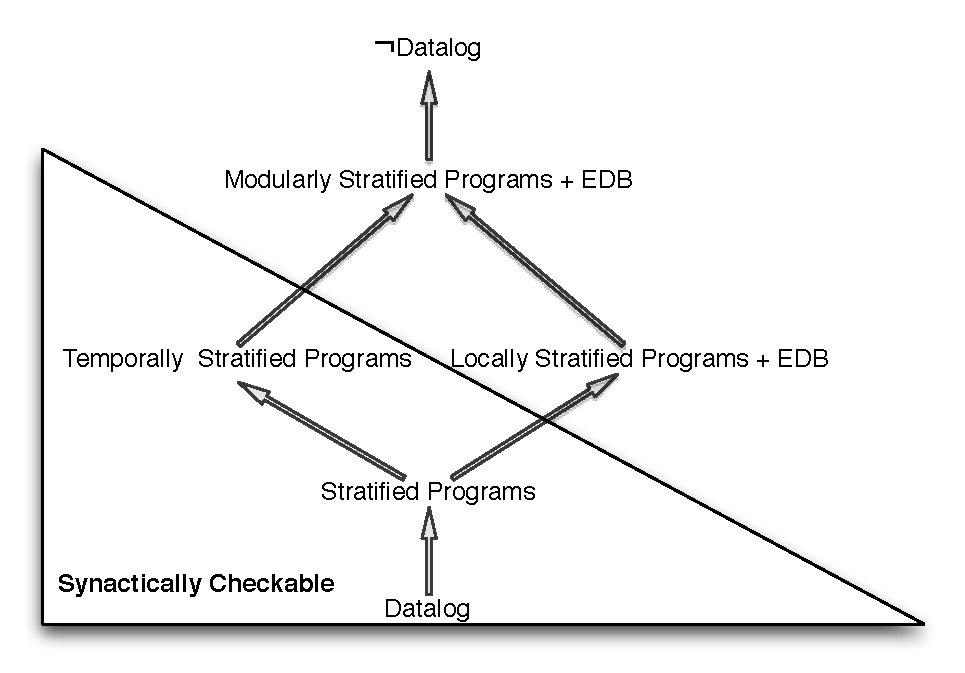
\includegraphics[width=0.75\linewidth]{figures/dedalus_classes.pdf}
  \label{fig:dedalus-classes}
  \caption{Stratifiability classes.  $A \to B$ means that every program in $A$ is in $B$.}
\vspace{-8pt}
\end{figure}


%%\paa{I don't think we can show that programs with async rules are locally stratifiable, actually}
%%\wrm{Why not?  What if we have that "causality constraint" we were talking about?}



\subsection{Temporal Safety}
A Datalog program is safe if it admits a finite minimal model, and hence has
a finite execution.  Safety in Datalog is traditionally achieved
through the following constraints:

\begin{enumerate}
%
\item No functions are allowed.
%
\item Variables are \emph{range restricted}: all attributes of the head goal
appear in a non-negated body subgoal.
%
\item The EDB is finite.
%
\end{enumerate}

These constraints ensure that the Herbrand Universe is finite: any atom that
may be deduced by a safe program may only take its attributes from the 
set of all constant symbols appearing in the program and EDB.
%%~\nrc{Don't know what this means, but I suspect it is fancy-pants language for no good reason.}
%%\paa{ignoring this provocative comment.}
%%\wrm{lol.}
In fact, the set of all possible assignments of these constants to predicate
attributes, representing every possible interpretation, is itself finite. 

Since our definition of \dedalus{successor} violates these rules, and indeed
leads to an infinite set of facts, \slang programs violate this
definition of safety.  However, \dedalus{successor} models time, not computation;
later sections explain how \lang implementations avoid enumerating the contents
of \dedalus{successor} at runtime.
%%\wrm{whats pailiative (helping fix the problem) here???}.  
This section
introduces a notion of termination that allows us to reason about the safety of
\slang programs.

%\nrc{Seems like there ought to be more here. Why do I care about the
%  preceding text? What does it have to do with the following text?}

%Since the Herbrand Universe is finite, any instantiation of predicates with
%constants is finite.  Every possible interpretation (set of ground atoms) of
%a logic program comes from this finite instantiation, so any possible
%interpretation is finite
  
%\paa{the idea is: safe=finite.  herbrand universe=finite, so any instantiation of predicates with constants is finite.
%every possible interpretation (set of atoms) of a LP comes from this instantition.  so any possible interpretation is finite.
%a model is an interpretation in which all heads are true when the body is true.  all models are finite.  the minimal model
%is clearly finite.}

%\subsection{Temporal Safety}

%%\wrm{show some examples before restricting to temporal safety!!  maybe even
%%show that some unsafe programs have safe equivalents.}

A \slang program containing only deductive rules is informally equivalent to a
Datalog program in which all predicates have no time suffix.  If all the rules
in such a program meet the conditions above, then clearly we would like them to meet \slang's definition of safety. 
%%\rcs{this used to say conditions 1 and 2, but it is possible that our program is infinitely long...  Also, ``clearly they are safe'' is strange, given that we haven't defined 
%%safety yet, so I reworded.}

\begin{definition} 
%
The \emph{deductive reduction} of a \slang program $P$ is
the subset of $P$ consisting of exactly the deductive rules in $P$.
%
\end{definition}

\begin{definition}
%
A rule is \emph{instantaneously safe} if it is deductive,  function-free and range-restricted.
A \slang program is instantaneously safe if its deductive reduction is instantaneously safe.
%
\end{definition}

%Inductive rules may be unsafe.  Consider the \dedalus{successor} relation described above.  According to our
%intuitive interpretation, this relation models the passage of time, in order to
%establish a temporal order among ground atoms. 

The \dedalus{successor} relation complicates the discussion of safety, as it
introduces the countably infinite set $\mathbb{Z}$ to our
%Herbrand
universe of constants.
%Clearly, a naive interpretation of time can lead to unsafe programs:
%\rcs{how is this any more unsafe than succ(x+1) :- succ(x)?  Suggested text:}

%The infinte \dedalus{successor} relation complicates our discussion of safety;
Consider the following \slang program, which derives a single, persistent fact:

%Consider the \dedalus{successor} relation described above.  According to our
%intuitive interpretation, this relation models the passage of time, in order to
%establish a temporal order among ground atoms. 
%%\wrm{we're ignoring entanglement here}
%Recall that {\em successor} is the standard strict total order on
%$\mathbb{Z}$, lol, don't know how I accidentally wrote the above incorrect
%sentence all over the paper
%Recall that \dedalus{successor} is an infinite relation.  Clearly, a naive
%interpretation of time can lead to unsafe programs:

%%No reason to re-define a strict total order here...
%\begin{itemize}

%\item $\forall A,B \in \mathbb{Z} : successor(A, B) \Rightarrow B > A$ (i.e. whenever $successor(A,B)$ is true, then $B > A$)

%\item $\forall A \in \mathbb{Z} : \exists! B \in \mathbb{Z} : successor(A,B)$ (i.e. every integer has a successor)

%\end{itemize}

%\wrm{we'd expect a lot more properties of successor than the ones you mentioned.  so instead of trying to think of them all, i just narrowed down what you wrote.}

%This implies that successor is infinite (as we'd expect time to be), and is problematic because it leads to unsafe programs.


\begin{example}
\label{ex:tempsafe}
%
An unsafe \slang instance?
\\
%%\begin{Dedalus}
%%p\pos(A, B)@next \(\leftarrow\) p\pos(A, B), \(\lnot\)p\nega(A, B);
%%\end{Dedalus}
\begin{Dedalus}
persist[p, 2]
p(1, 2)@123;
\end{Dedalus}

%%\paa{we shouldn't \emph{ever} need to write out r2, right?}

The single ground fact will cause one deduction for each tuple in
\dedalus{successor}.  Since \dedalus{successor} is infinite, the corresponding
Datalog
%%\rcs{what should we call this?}
program is unsafe.  
%
\end{example}

However, observe that each of these deductions produces a tuple that changes
only in its time suffix.  We find it useful to distinguish between unsafe
programs and programs that, given a finite EDB, eventually derive only tuples
that are equivalent except in their time suffixes.

%%\wrm{$<$don't really get whats going on$>$}
%%Consider a \emph{derivation tree} as defined by Levy et al~\cite{levy}.  
%%\paa{he's halevy now.  should it be halevy et al?  or is that confusing?  I blame alon.}
%%According to their definition,
%%two goal nodes $g_1$ and $g_2$ are \emph{identical} if they have the same predicate symbol and, in each argument
%%position, the same variables.  Two nodes are \emph{equivalent} if there exists a one-to-one mapping
%%$\phi$ from $V(g_1) \to V(g_2)$ such that $\phi(g_1) = g_2$.


%%\paa{I may have made a mess of this.  derivation trees are probably more machinery than we need to describe, for
%%the purposes of the definition of a 'stable inference', the 1-step deduction of an atom from another atom having the same
%%name and the same values for all attributes but time}
%%\wrm{I still don't know why we need to use derivation trees here.}
%%\wrm{Define 'derivation'.  Joe sez: "Here I think you just need an appropriate reference for derivation trees, along with some simple intuition.  I believe the right ref is %%"Constraints and Redundancy in Datalog", Levy/Sagiv, PODS 92."}

%%\begin{definition}
%%An \emph{inference} is a single step in a derivation, corresponding to a goal node, its child rule node, and the child goal
%%nodes of this rule node.  
%%\end{definition}

%%\paa{or... ditch all this stuff about derivations, define an 'inference' as a single deduction of an atom from established atoms;
%%ie the single evaluation of a rule, and proceed from here with the definitions}

%%\textbf{alternate derivation-free definition:}
%%\begin{definition}
%%An \emph{inference} is the deduction of an atom from established atoms via the application of a rule.
%%\end{definition}
%%\wrm{what's a rule application?}

%%\begin{definition}
%%A \emph{stable inference} has a goal $\gamma'$ with time suffix $\Tau$ derived
%%from a child goal $\gamma$ with time suffix $\Tau-1$, such that $\gamma$ differs from
%%$\gamma'$ only in its time suffix.
%
%%\end{definition}

%%In other words, $\pi_\xi(\gamma')$ is equivalent to $\pi_\xi(\gamma)$, where $\xi$ is the set of attributes in $\gamma$
%%minus $\Tau$.\wrm{$<$/dont really get whats going on$>$}.

%%\wrm{How about we delete everything above and just say this:}

%%To distinguish between programs that 
%%produce these infinite \emph{void inductions} and those that correspond 
%%intuitively to the Datalog notion of unsafe programs, we introduce the concept of
%%\emph{temporal safety}.

%%\begin{definition}
%%An intensional predicate $e$ in a program $P$ is called an \emph{event predicate} if there exist
%%in $P$ no rules with $e$ in their head. \wrm{how is this different from an EDB predicate??}
%%\end{definition}

\begin{definition}
%
Two sets of ground atoms $\Gamma$ and $\Gamma'$ are \emph{equivalent modulo
time} if each atom $\gamma \in \Gamma$ has a corresponding atom $\gamma' \in
\Gamma'$ such that $\gamma$ and $\gamma'$ have the same predicate symbol, and
the same assignment of constants to attributes for all attributes except the
time suffix.
%
\end{definition}

%%In other words, $\pi_\xi(\gamma')$ is equivalent to $\pi_\xi(\gamma)$, where $\xi$ is the set of attributes in $\gamma$
%%minus $\Tau$.\rcs{either define pi, write out ``projection'', or drop this paragraph}

\begin{definition}
%
We say a \slang instance is \emph{quiescent at time $T$} if the set of all
atoms with time suffix $T$ is equivalent modulo time to the set of all atoms
with time suffix $T-1$.
%%\rcs{what is a true atom?  Why distinguish between true atoms and false atoms?  Surely the neg tuples will match as well.  If not, then the program has somehow not quiesced...}
\end{definition}

%%\paa{well, there are some problems with this.  first, facts are only in the EDB, you mean atom,
%%second, this is never true because of the time suffix (unless you mean to have defined ``fact''
%%precisely as $\pi_\xi(p)$ for any predicate p.)  what I was trying to do was define quiescence in terms
%%of inference; a quiescent DB is one for which all inferences are stable.}

\begin{observation}
%
A \slang instance that is quiescent at time $T$ will be quiescent until
timestamp of the next EDB fact $V$, i.e. for all $U \in \mathbb{Z}: V > U >=
T$.  If no EDB fact has a timestamp greater than $T$, then the instance will be
henceforth quiescent.
%%\rcs{what does it mean for an edb fact to be true at time $T$?  It would be better to say that there is no EDB fact with timestamp T, since we're trying to ground the discussion without talking about time.}
%
\end{observation}
%
\begin{proof}
%
%%\wrm{sightly ???}
A \slang program admits only instantaneous and inductive rules, which derive
new tuples at the same time as their ground tuples, or in the immediate next
timestep.  Thus, the set of tuples true at time $T$ is completely determined by
any tuples true at time $T-1$, and any EDB facts true at time $T$.  Observe
that the integer value of the timestep does not influence the derivation.

If the instance is quiescent at $T$, then given ${\bf A}$, the set of atoms
with timestamp $T-1$, and the EDB at $T$, the program entails ${\bf
A}$ at timestamp $T$.  Thus in the absence of EDB facts at $T+1$, it entails
${\bf A}$ at $T+1$.
%
\end{proof}

\begin{definition}
%
A \slang instance with finite EDB is \emph{temporally safe} if it is henceforth
quiescent after some time $T$.
%
\end{definition}
%%\wrm{the following doesn't seem like a definition, seems more like a test for temporal safety}
%%\begin{definition}

\begin{definition}
%
Given the depends-on relation $\succ$ and its transitive closure $\succ^{*}$,
an intensional predicate $e$ in a program $P$ is called an \emph{instantaneous
predicate} if for every predicate $p$ for which $e \succ^{*} p$ (ie, $e$
depends transitively on $p$), either $p$ appears in the head of no inductive rules, or the body
of each inductive rule with head $p$  contains at least one positive instantaneous 
predicate.

\end{definition}

%%A rule is temporally safe if:
We propose the following conservative test for temporal safety.  A program is
guaranteed to be temporally safe if every rule is either:

\begin{enumerate}
%
\item An instantaneously safe rule, or
%
\item An inductive rule in which the head predicate occurs also in the
body with the same variable bindings for all attributes save the time suffix,
or
%%occurs also in the body with the same assignment of variables and constants to attributes.
%
\item An inductive rule that has at least one instantaneous predicate as a
positive subgoal in the body.
%
\end{enumerate}

%%\paa{maybe this is too greedy.  rule 1 above defines "instantaneous safety" or classical datalog-type safety.  
%%if all deductive rules respect rule 1, we are instantaneously finite.  the other two rules describe temporal safety
%%as such.  that is to say: any deductive rule that is range-restricted and function-free is instantaneously safe (deductive rules do
%%not reference the infinite relation \emph{successor}.  instantaneously safe <=> safe in datalog) further, any instantaneously safe rule is temporally safe.  
%%also, rules that are (2,3) are temporally safe.}

While a temporally safe program is henceforth quiescent after some time $T$,
a temporally unsafe program changes infinitely.  Note that
the \slang program in Example~\ref{ex:tempsafe} is temporally safe because
\emph{r1} satisfies the second condition above.

\begin{lemma} 
%
A temporally stratifiable \slang instance with finite EDB where every rule is
one of the kinds 1-3 above is indeed temporally safe.
%
\end{lemma}
%
\begin{proof}
%
Assume the program is temporally unsafe.  That is, there exists no time $T$
such that $\forall U >= T$, the set of all atoms with timestamp $U$ is
equivalent modulo time to the set of all atoms with timestamp $T-1$.  Let $E$
be the maximum timestamp of any fact in the EDB.

Observe that every rule $r$ of kind 3 may only entail a finite number
of facts---as the EDB is finite---and thus may entail no facts at a
timestamp greater than some maximum timestamp $V_r <= E+1 \in
\mathbb{Z}$.  Since a \slang program has a finite set of rules we know
$\exists V \in \mathbb{Z} : \forall r: V >= V_r$, and thus $V <= E+1$.

We now consider times $T$ such that $T > E+1$.  By the above argument, no rules
of kind 3 entail any facts with a timestamp greater than $E+1$.  Recall that
no EDB atoms are true at any timestamp greater than $E$.  Thus, any facts with
timestamp greater than $E+1$ are entailed by rules of kind 1 or 2.

Consider the set of equivalence classes modulo time of all possible atoms, {\bf
A}, given the Herbrand universe.  We know {\bf A} is finite, as the Herbrand
Universe is finite.  Therefore, if the program is temporally unsafe, then {\bf B}, the
set of atoms entailed by the program, both contains and excludes
infinitely many members of at least one equivalence class in {\bf A} (i.e.
something ``infinitely oscillates in time'' between being true and false).
Since the program has finitely many rules, at least one rule must entail
infinitely many atoms (from at least one of the equivalence classes from {\bf
A}). Thus, it is easy to see that there must be a cycle that contains some predicate $P$ and $\lnot P$.

We show there exists such a cycle containing only rules of kind 1, which
implies that the program is temporally unstratifiable.  In order for such a
cycle to exist, $P$ must transitively depend on $\lnot P$, and $\lnot P$ must
transitively depend on $P$.  Thus, the program contains a rule $J_1$ with
$\lnot P$ in its body, and some predicate $R$ in its head, as well as a rule
$J_2$ that is transitively dependent on $R$, with $P$ in its head.

{\bf Case 1: }$P \neq R$.  In this case, $J_1$ must be of kind 1, as for any $Q
\neq P$, a rule of kind 2 with $P$ in the head may not directly entail $Q$
given $P$.  $J_2$ must also be of kind 1---if it is of kind 2, then it
necessarily contains $P$ in its body, so it cannot entail $P$ unless $P$ is
entailed by some other rule.  If $J_2$ contains $R$ in its body, then the
program is syntactically unstratifiable.  But if $J_2$ does not contain $R$ in
its body, then it contains some predicate $S$ transitively entailed by $R$;
wlog the body contains $R$.  Thus, the program is syntactically unstratifiable.

{\bf Case 2: }$P = R$.  In this case, $J_1$ and $J_2$ are the same rule: $P
\leftarrow \lnot P$.  Thus, the program is syntactically unstratifiable.

Thus, the program is temporally unstratifiable, which contradicts our
assumption.
%
\end{proof}

\begin{example}
A \slang instance with a temporally unsafe deductive rule.
%%\rcs{is this even a \slang instance?  Is it a Datalog instance?  Perhaps this example belongs earlier in the text, where we define range-restricted.}


\begin{Dedalus}
p(A, B) \(\leftarrow\) q(A);
\end{Dedalus}

The program above has a temporally unsafe deductive rule that corresponds to an
unsafe rule in Datalog: it is not range-restricted.  The head variable $B$
could range over an infinite set of constants.
\end{example}


\begin{example} 
%
A \slang instance that is temporally unsafe due to infinite oscillation.

\begin{Dedalus}
flip\_flop(B, A)@next \(\leftarrow\) flip\_flop(A, B);
flip\_flop(0, 1)@1;
\end{Dedalus}

The above program exemplifies temporally unsafe induction. Even though it
contains no function symbols, and all variables are range-restricted, it
entails infinite oscillation of the \emph{p} predicate.  
%because the \emph{p} predicate occurs in the head with a different variable
%binding than in the body, and because there are no positive event predicates
%in the body.  
%%\wrm{this makes me a bit uncomfortable.
%%we've defined a conservative test for temporal safety.  so if something fails
%%the test, it's not necessariliy temporally unsafe.}
\end{example}

We can imagine interesting examples of temporally unsafe programs, and do not forbid them
in \slang. 
%%\wrm{joe sez "discuss safety is wil, but-out regured"}

%%By providing a conservative syntactic check for temporal safety, we ensure that \slang
%%programs have 

%An inductive rule cannot cause infinite oscillation if it has a positive event predicate in its body, because we are assuming a finite EDB.

%%However, we observe that all of these deductions are uninteresting, as they are
%%deterministically related to the EDB.  To avoid performing such deductions, we
%%restrict {\em successor} to range over the subset of $\mathbb{Z}$ consisting of
%%the consecutive natural numbers between the minimum and maximum timestamp
%%specified in the (finite) EDB ($\{123, 124\}$ in this example) \wrm{this is without NDB right?}.  If we extended the EDB with the additional facts:

%But if \emph{successor} is infinite, many of these deductions may be \emph{void}in some sense, i.e. functionally determined based on the EDB. \wrm{is functionally determined a real term?}
%In effect, an EDB that is given in its totality determines a window over successor that is relevant to any computation that must be performed.  \wrm{what about NDB?}
%It is easy to see that in this example, we need only consider a successor relation that contains a single tuple \{123, 124\}.

%%\begin{Dedalus}
%%delete p(1, 2)@456;
%%p(?, ?)@789; \wrm{we're still doing queries?}
%%\end{Dedalus}

%%Evaluating the \lang instance would require \emph{successor} to range over the
%%subset of consecutive natural numbers $[123, 790]$.

%%\begin{definition}
%%A \emph{post-hoc} evaluation is an evaluation of a \lang instance where
%%{\em successor} ranges over the finite subset of $\mathbb{Z}$ described above.
%%\end{definition}

%%In a post-hoc evaluation, we can derive {\em successor} from the EDB as part of
%%the fixpoint computation.  We first define a predicate \emph{event\_time} that
%%contains the union of the time attributes from the EDB:

%%$event\_time(\Tau) \leftarrow \displaystyle\bigvee_{p \in EDB} p([...], \Tau)$

%%\wrm{I wasn't a fan of expressing a query plan in a Datalog rule...  But we can
%%talk about this}

%%We then populate \emph{successor} with \lang program shown below:
%with arithmetic and aggregate functions, as shown below.

%%\begin{Dedalus}
%%smax(max<N>) \(\leftarrow\) event\_time(N);
%%smin(min<N>) \(\leftarrow\) event\_time(N);

%%successor(N, N + 1) \(\leftarrow\) smin(N);

%%successor(S, S + 1) \(\leftarrow\) 
%%    successor(N, S),
%%    smax(M),
%%    N <= M;
%%\end{Dedalus}

%%\wrm{Not sure what the point of this is...}
%%Since {\em successor} is finite in a post-hoc evaluation, we may evaluate the
%%ntire \lang instance in a single fixpoint.

%In a post-hoc evaluation, time is in some sense ``instantaneous" in that all values of the successor relation are considered in a single
%fixpoint computation.  The complete program is safe if the EDB is finite.



%%
\subsection{Stratification in {\large{\bf\slang}}}
\label{sec:strat}
We first turn our attention to the semantics of
programs with negation.  As we will see, the inclusion of time enables
programs' local stratification, and the existence of a unique perfect model
that corresponds to intuition. \wrm{reword}

%``source of monotonicity''  a unique perfect model

%semantics in some surprising cases, and enables purely syntactic monotonicity
%checks for a broad class of temporal programs.

%%\paa{notes}

%%this section has become cluttered, but for me the main results are the following:

%%\begin{enumerate}
%%\item Negation-, aggregation- and choice-free \lang programs have a unique minimal model (pure Datalog)
%%\item stratifiable \lang programs have a unique minimal model (again, Datalog, but we need to show that the restrictions and syntactic transformations
%%cannot introduce a cycle or add a negative edge to an existing cycle.)
%%\item \emph{temporally stratified} \lang programs (w/o choice) force any cycles with negation to involve an inductive edge, forcing an ordering on the evaluation.
%%we can show that in all such cases, the corresponding datalog program is modularly stratified (insofar as \emph{successor} is considered to be ``completely
%%evaluated" in a lower module.)  since modularly stratified programs have a unique stable model, so do any temporally stratified \lang programs.
%%\end{enumerate}

\begin{lemma} \label{lemma:no-neg-unique}
%
A \slang program without negation 
%%and aggregation 
has a unique minimal model.
%
\end{lemma}

\begin{proof} 
%
A \slang program without negation 
%%and aggregation 
is a pure Datalog
program.  Every pure Datalog program has a unique minimal model. 
%
\end{proof}

%%\jmh{Oops, you forgot that this model is countably infinite due to infinite time. So I could add countably many random consistent facts and have an equally ``small'' model. You will need a more refined definition of safety and minimality that accounts for time.}

%%\jmh{I'm going to stop commenting here since you'll need some more machinery to continue.}

We define syntactic stratification of a \slang program the same way it is
defined for a Datalog program:

\begin{definition}
%
A \slang program is \emph{syntactically stratifiable} if there
exists no cycle with a negative edge 
%%or an aggregation edge 
in the program's
predicate dependency graph.
%
\end{definition}

%%We evaluate such a program by evaluating each strongly connected component of
%%its predicate dependency graph under a closed-world assumption.  

We may evaluate such a program in {\em stratum order} as described in the
Datalog literature~\cite{ullmanbook}.
%%\wrm{cite?}
%any order returned by a topological sort on the predicate dependency graph,
%with each strongly connected component collapsed to a single node.
It is easy to see that any syntactically stratified \slang instance has a
unique perfect model \wrm{cite?} because it is a syntactically stratified Datalog program.

%\begin{lemma}
%
%A syntactically stratifiable \lang instance without choice has a unique
%minimal model.  That is, there exists a function $D$ from syntactically
%stratifiable \lang instances without choice to their minimal models.
%
%\end{lemma}

%\begin{proof}
%\wrm{todo: insert statement that this is obvious}
%
%We know that there exists a function $B$ from syntactically stratifiable
%Datalog instances to their minimal models \wrm{cite?}.  Earlier, we introduced
%\wrm{XXX: where?} a bijection \wrm{XXX: probably not a bijection} $A$ from the
%set of \lang instances without choice to the set of Datalog instances, and a
%bijection $C$ between minimal models of Datalog instances and minimal models of
%\lang instances without choice.  We will show that $D = C \circ B \circ A$.

%Thus, we need only prove that the restriction of $A$ to syntactically
%stratifiable \lang instances without choice maps to a subset of syntactically
%stratifiable Datalog instances.  But this is clear, as $A$ does not add any
%rules to the instance, and may introduce only the non-negated EDB {\em
%successor} relation to the body of an existing rule.  Thus, $A$ cannot
%introduce any new cycle or add negation to any existing cycle in the instance's
%predicate dependency graph.
%
%\end{proof}

However, many programs we are interested in expressing are not syntactically
stratifiable.  Fortunately, we are able to define a syntactically checkable
notion of {\em temporal stratifiability} of \slang programs that maps to a
subset of {\em locally stratifiable} \wrm{cite, and mention this term was coined previously} Datalog programs.

%Intuitively, a Datalog instance is modularly stratifiable if no EDB
%element depends negatively on itself.

%%\begin{example}
%%Consider a predicate \emph{print} that corresponds to a print queue.  The program below
%%states that if there is a message \{A, B\}, then there 
%%\begin{Dedalus}
%%print(A, B) \(\leftarrow\)
%%  message(A, B),
%%  \(\lnot\)print(A, B);
%%\end{Dedalus}
%%\end{example}

%Peter said we might not need these formal definitions.  Experimenting without
%\begin{definition}
%
%A Datalog program and EDB is \emph{locally stratifiable} if, after
%instantiating the rules given the Herbrand saturation of the program and EDB,
%there exists no cycle with a negation or aggregation edge in the dependency
%graph of instantiated ground atoms.
%
%\end{definition}

%We take the definition below from Ross~\cite{modular, ross-syntactic}.
%\begin{definition}
%
%A Datalog instance is \emph{modularly stratifiable} if, and only if its
%mutally recursive components are locally stratified once all instantiated rules
%with a false subgoal that is defined in a ``lower" component are removed.
%\end{definition}

%\begin{lemma}
%
%A locally stratifiable \lang instance without choice has a unique
%minimal model.  That is, there exists a function $E$ from locally
%stratifiable \lang instances without choice to their minimal models.
%
%\end{lemma}

%\begin{proof}
%
%\wrm{TODO}
%
%\end{proof}


\begin{definition} 
%
The \emph{deductive reduction} of a \slang program $P$ is
the subset of $P$ consisting of exactly the deductive rules in $P$.
%
\end{definition}

\begin{definition} 
%
A \slang program is \emph{temporally stratifiable} if its deductive
reduction is syntactically stratifiable.
%
\end{definition}

\wrm{major false depth here, I say we eliminate the theorem and just cite
Datalog/UT here: ``This paper has shown that by making the local stratification
of programs explicit in time stamps a pure logical theory of updates is
possible.''}

%%\newtheorem{theorem}{Theorem}
\begin{lemma}
\label{lemma:temp-strat-uniq}
%
Any temporally stratifiable \slang instance $P$ has a unique perfect model.
%
\end{lemma} 

\begin{proof}
%
{\bf Case 1:} $P$ consists of only deductive rules.  In this case, $P$'s
deductive reduction is $P$ itself.  We know $P$ is syntactically stratifiable,
thus it has a unique perfect model.

{\bf Case 2:} $P$ consists of both deductive and inductive rules.  Assume that
$P$ does not have a unique perfect model.  \wrm{and the proof requires a bit of
touching up here...}

This implies that $P$ is not
syntactically stratifiable.  Thus, there must exist some cycle through at least
one predicate $q$ involving negation.
%%or aggregation.  
Furthermore, this cycle must involve an inductive rule, as $P$ is temporally
stratified.

Since the time suffix in the head of an inductive rule is strictly greater than
the time suffix of its body, no atom may depend negatively on itself---it may
only depend negatively on atoms in the previous timestep.  Thus, $P'$ is
{\em universally contraint stratified} because induction through time implies a
monotonicity constraint \wrm{cite Ross}.  This guarantees a unique perfect model
achievable via standard bottom-up fixpoint execution.
%
%does not have a unique minimal model.  This implies that $P$ is not
%syntactically stratifiable, thus there must exist some cycle through at least
%one predicate $q$ involving a negation or aggregation edge in $P$'s predicate
%dependency graph, and furthermore this cycle must include at least one
%inductive rule.  Since an inductive rule has a time suffix $S := N+1$, where
%$N$ is the timestamp of its body, and $P$'s deductive reduction is
%syntactically stratifiable, we know that the aggregate or negation of $q$ must
%always occur in a strictly earlier or later timestamp than that of the
%positive $q$ atom.  Since the timestep in the cycle increases monotonically
%with each iteration, $q$ will never, in practice, depend on a negation or
%aggregate of itself.  Thus, $P$ is locally stratifiable, and by Lemma XXX
%above, $P$ has a unique minimal model.  This contradicts our assumption that
%$P$ does not have a unique minimal model.  Thus, $P$ has a unique minimal
%model.
%
\end{proof}


\begin{example}
A simple temporally stratifiable \slang program that is not syntactically stratifiable.

\begin{Dedalus}
persist[p, p\_neg, 3]  
  
r1
p(A, B, T) \(\leftarrow\)
  insert\_p(A, B, T);

r2  
p_neg(A, B, T) \(\leftarrow\)
  p(A, B, T),
  delete\_p(T);
\end{Dedalus}

In the \slang program above, \emph{insert\_p} and \emph{delete\_p} are captured
in EDB relations.  This reasonable program is unstratifiable because $p \succ
p\nega \land p\nega \succ p$.  But because the successor relation is
constrained such that $\forall A,B, successor(A, B) \rightarrow B > A$, any
such program is locally stratified on time suffixes.  Therefore, we have
$p_{n} \not\succ^* p\_neg_{n} \not\succ^* p_{n+1}$; informally, earlier values
do not depend on later values.
%%\paa{need to make the text better, but this old example probably makes sense here}
\end{example}

\begin{figure}[t]
  \centering
  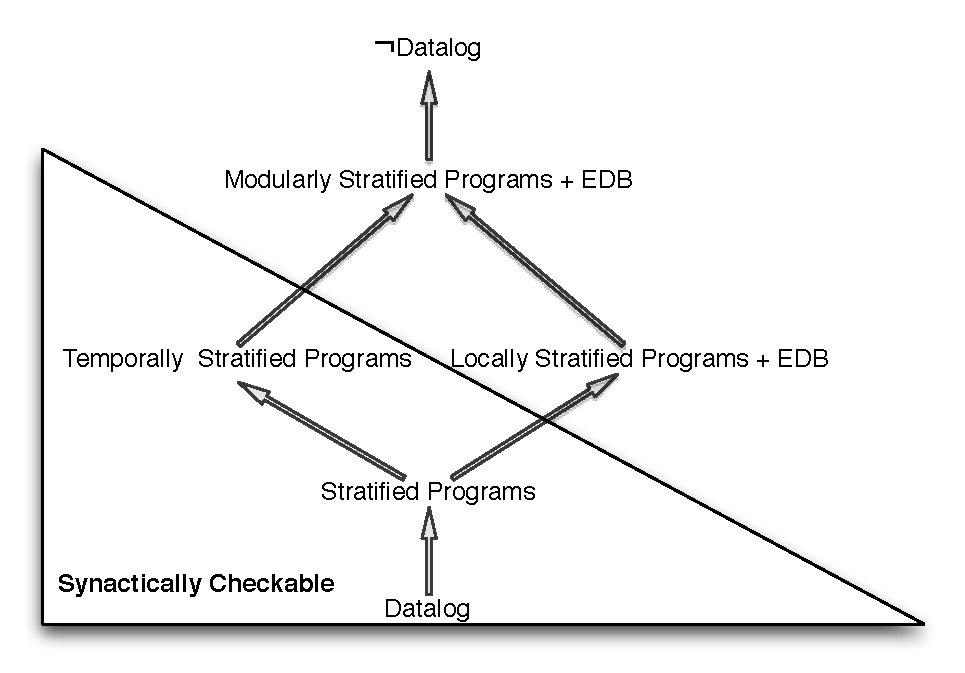
\includegraphics[width=0.75\linewidth]{figures/dedalus_classes.pdf}
  \label{fig:dedalus-classes}
  \caption{Stratifiability classes.  $A \to B$ means that every program in $A$ is in $B$.}
\vspace{-8pt}
\end{figure}


%%\paa{I don't think we can show that programs with async rules are locally stratifiable, actually}
%%\wrm{Why not?  What if we have that "causality constraint" we were talking about?}


\section{Cost Model}

%%\newdef{definition}{Definition}
Lemma~\ref{lem:cost} expresses that we can trade computation cost for storage 
cost in evaluation of a Dedalus program. 

%In the continuous interpretation of a Dedalus program, it is in general only
%useful to remember facts at a single timestamp in a predicate.  Two ways to
%approach this issue are to either always persist the ``latest'' version, or
%continuously re-derive the latest version.  These are represented in the naive
%deductive and overwriteable storage implementations below.

%\begin{figure}[t]
%\begin{tabular}{ll} \hline
%%Rule Pattern & Idiom & Prepare & Propose & Election \\ \hline \hline
%$d$ & Cost of a deductive step \\
%$s$ & Cost of storing a tuple \\
%$r$ & Cost of reading a tuple \\ 
%$t$ & Number of tuple derivations from deductive rules \\ 
%\hline
%$S$ & Set of tuples inserted \\
%$U$ & Set of tuples updated \\
%$P$ & Set of stored tuples, with time projected out \\ 
%$T$ & Set of stored tuple timestamps \\ 
%$Q$ & Set of query timestamps \\ \hline 
%\end{tabular}
%\caption{Cost model.}
%\label{fig:breakdown}
%\end{figure}


\subsubsection{Naive Deductive Implementation}

To evaluate a trace consisting of $S$ inserts and $U$ updates, a naive
deductive implementation would:

\begin{enumerate}

\item Add all inserts, deletions, and updates to the EDB.  
%We make the simplifying assumption that all EDB predicates are indexed by some
%hash of their key attributes.
Note that an update consists of both an insertion and a deletion.  Assuming
that inserting a fact into the EDB has some cost $w$ independent of the
characteristics of the predicate (e.g. all predicates store their facts in hash
tables), then the cost of this step is $(S+2U)w$.

\item For every predicate $P$, at time $M$, we must evaluate all predicates in
$P$'s predicate dependency graph at time $1$ through $M$.  
%A bottom-up evaluation of a predicate $P$ consists of evaluating all rules
%that reference $P$ in the head, and may involve polynomially many derivations
%in the size of the EDB up to time $M$.
A naive query plan for execution of a rule would consist of taking the cross
product of all body relations, selecting the subset that matches the body
conditions, and projecting this subset onto the head predicate to derive new
head tuples.  Assume each rule has an associated
selectivity $s_r$ and cost per each tuple in the join result $d_r$.  If a rule
is part of a recursion, it will be executed for $n_r$ steps.  The cost
of this evaluation is $M \cdot \sum_{r} n_r \cdot s_r \cdot d_r$.

\end{enumerate}

In summary, the total execution cost is:

\[ (S+2U)w + M \cdot \sum_{r : P \in r.head} n_r \cdot s_r \cdot d_r  \]

Since we only need persist the EDB, the total storage cost is equal to the size
of the EDB.

%$(|S|+2|U|)s + (|S|+2|U|)r + t + (\displaystyle\sum_{i=0}^{|Q|-1} \displaystyle\sum_{j=0}^{|T|-1} Q_{i} - T_{j})d$

\subsubsection{Naive Overwriteable Storage Implementation}

An overwritable storage implementation may enable lower execution latency by
storing the most recent version of a tuple.  For a predicate $P$ at time $M$,
we would need to evaluate each predicate $Q$ in $P$'s predicate dependency
graph from timestamp $Q_N+1$ through timestamp $M$ -- where $Q_N$ is the
timestamp of the last stored tuple of predicate $Q$. This is in contrast to the
naive deductive model, which would require computation from timestamp 1, but
would not require persisting the IDB of the most recently computed stratum for
each predicate.

In summary, the total execution cost is:

\[ (S+2U)w + \sum_{r} (M - Q_{r.head}) n_r \cdot s_r \cdot d_r  \]

The total storage cost is the IDB of each predicate at its most recent
timestamp.

%%\subsubsection{perhaps we can admit queries over the past that are bounded and pre-stated, and do GC}

\section{Asynchrony}
\label{sec:async}

% \begin{figure}[t]
%   \centering
%   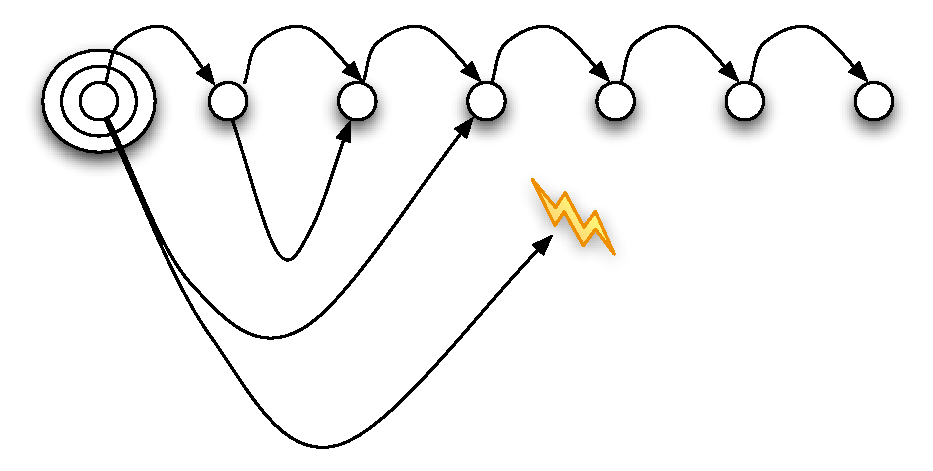
\includegraphics[width=0.75\linewidth]{figures/dedalus-time.pdf}
%   \label{fig:time}
%   %%\caption{Time moves forward in three ways: across strata, to the next fixpoint, and to some future fixpoint.}
%    \caption{Dedalus admits inferences whose consequences are visible immediately, in the next timestep, or at some unspecified timestep.}
%    
% \vspace{-8pt}
% \end{figure}

In this section we introduce \lang, a superset of \slang that also admits the
\emph{choice} construct~\cite{greedychoice} to bind time suffixes.  Choice
allows us to model the inherent nondeterminism in communication over unreliable
networks that may delay, lose or reorder the results of logical deductions.  We
then describe a syntactic convention for rules that model communication between
agents, and show how \lang can be used to implement common distributed computing
idioms like Lamport clocks and reliable broadcast.

\subsection{Choice}

%%In this section we present the Datalog extensions missing from \slang that we will need in \lang to capture important properties of practical distributed systems.  These include aggregate functions to 
%%capture ordering constraints, and---more importantly---the choice construct to capture nondeterminacy.


%%\subsubsection{Choice}
An important property of distributed systems is that individual computers cannot control or observe the temporal interleaving of their computations with other computers.  One aspect of this uncertainty is captured in network delays: the arrival ``time'' of messages cannot be directly controlled by either sender or receiver.  In this section, we enhance our language with a traditional model of nondeterminism from the literature to capture these issues: the \emph{choice} construct as defined by Greco and Zaniolo~\cite{greedychoice}.

The subgoal \dedalus{choose((\emph{$X_1$}), (\emph{$X_2$}))} may appear
in the body of a rule, where \emph{$X_1$} and \emph{$X_2$} are vectors
whose constituent variables occur elsewhere in the body.  Such a
subgoal enforces the functional dependency \emph{$X_1$} $\to$ $X_2$,
``choosing'' a single assignment of values to the variables in
\emph{$X_2$} for each variable in \emph{$X_1$}.

The choice construct is nondeterministic.  In a model-theoretic interpretation of logic programming, a nondeterministic program 
must have a multiplicity of {\em stable models}---that is, it must be unstratifiable.  
Greco and Zaniolo define 
choice in precisely this fashion: the choice construct is expanded into an unstratifiable strongly-connected component of rules, 
and each possible choice is associated with a different model.  Each such model has a unique, non-deterministic assignment that
respects the given functional dependencies.  In our discussion, it may be helpful to think of one such model chosen non-deterministically---a non-deterministic ``assignment of timestamps to tuples.''

%%\paa{significantly, for any choice, the resulting program has a unique minimal model if the program (independent of the choice expansion)
%%is stratifiable, locally stratifiable, etc}  \jmh{You do need to resolve the previous paragraph, or rewrite it to simply say ``see the Italians if you want to understand more, 
%%but for our purposes assume a unique non-deterministic assignment that respects the FDs.  This allows us to have agreed-upon minimal models.''}

\subsection{Distribution Model}
The choice construct captures the non-determinism of communicating agents in a distributed system, but we want to use it in a stylized way to model typical notions of distribution.  To this end, \lang adopts the ``horizontal partitioning'' convention introduced by Loo et al.~\cite{Loo:2005}.
To represent a distributed system, we consider some number of agents,
each running a copy of the same program against a disjoint subset ({\em
  horizontal partition}) of each predicate's contents.  We require one
attribute in each predicate to be used to identify the
partitioning for tuples in that predicate. We call such an
attribute a {\em location specifier}, and prefix it with a
\dedalus{\#} symbol in Dedalus.

Finally, we constrain \lang rules so that the location specifier variable in each body predicate be the same---i.e., the body contains tuples from exactly one partition of the database, logically colocated (on a single ``machine'').  If the head of the rule has the same location specifier variable as the body, we call the rule ``local,'' since its results can remain on the machine where they are computed.  If the head has a different variable in its location specifier, we call the rule a {\em communication rule}.  We now proceed to our model of the asynchrony of this communication, which is captured in a syntactic constraint on the heads of communication rules.

\subsection{Asynchronous Rules}

In order to represent the nondeterminism introduced by distribution, we admit a
third type of rule, called an {\em asynchronous} rule.  A rule is asynchronous
if the 
%Recall our use of the distinguished variables $\Tau$ and $S$ to represent the
%time suffixes respectively in the body and head of a rule
%(Section~\ref{sec:syntaxrestrictions}).  in our discussion of \slang,
%representing the time suffixes occuring respectively in the body and head of a
%rule.
relationship between the head time suffix $\SDedalus$ and the body time suffix $\Tau$ is
unknown.  Furthermore, $\SDedalus$ (but not $\Tau$) may take on the special value
$\top$ which means ``never.''  Derivation at $\top$ indicates that the
deduction is ``lost,'' as time suffixes in rule bodies do not range over
$\top$.

We model network nondeterminism using the choice construct to choose
from a value in the special 
%%\dedalus{successors} 
\dedalus{time}
predicate, which is defined using the following Datalog rules:

\begin{Dedalus}
time(\(\top\));
time(\(\SDedalus\)) \(\leftarrow\) successor(\(\SDedalus\), _);
\end{Dedalus}

\noindent
Each asynchronous rule with head predicate \dedalus{p($A_1, \ldots, A_n$)} has the following additional subgoals in its
body:

\dedalus{time($\SDedalus$), choose(($A_1, \ldots, A_n, \Tau$), ($\SDedalus$))}, 

\noindent
where
$\SDedalus$ is the timestamp of the rule head.  Note that our use of \dedalus{choose} incorporates all variables of each head predicate tuple, which allows a unique choice of $\SDedalus$ for each head tuple.


\begin{example}
A well-formed asynchronous \lang rule:

\begin{Dedalus}
r(A, B, \(\SDedalus\)) \(\leftarrow\) 
  e(A, B, \(\Tau\)),
  time(\(\SDedalus\)), choose((A, B, \(\Tau\)), (\(\SDedalus\)));
\end{Dedalus}
\end{example}

We admit a new temporal head annotation to sugar the rule above.  The
identifier \dedalus{async} implies that the rule is asynchronous, and stands in for
the additional body predicates.
%%$N$ is a variable,
%%corresponding to the time suffix $\Tau$ of all predicates in the rule body and
%%optionally referenced in the head.  
The example above expressed using \dedalus{async} is:

% asynchronous
\begin{example}
	A sugared asynchronous \lang rule:
	
\begin{Dedalus}
r(A, B)@async \(\leftarrow\) e(A, B);
\end{Dedalus}
\end{example}

\subsection{Asynchrony and Distribution in {\large{\bf\lang}}}
As a syntactic constraint of \lang, the {\em communication rules} introduced in the previous section (rules that differ in head and body location specifiers) are required to be asynchronous.
This restricts our model of communication between agents in two important ways.
First, by restricting bodies to a single agent, the only communication
modeled in \lang occurs via communication rules.  Second, because
all communication rules are asynchronous, agents may only learn about
time values at another agent by receiving messages (with unbounded
delay) from that agent.  Note that this model says nothing about the
relationship between the agents' clocks; they could be
non-monotonically increasing, or they could respect a global order.

\subsection{Temporal Monotonicity}
Nothing in our definition of asynchronous rules prevents tuples in the
head of a rule from having a timestamp that precedes the timestamp in
the rule's body. This is a significant departure from \slang, since it
violates the monotonicity assumptions upon which we based 
%both Algorithm~\ref{alg:tsn} and
our proof of
temporal stratification.  On an intuitive level, it may also trouble
us that rules can derive head tuples that exist ``before'' the body
tuples on which they are grounded; this situation violates intuitive notions of
causality and admits the possibility of temporal paradoxes.

We have avoided restricting \lang to rule out such issues, as doing so
would reduce its expressiveness.  Recall that simple monotonic Datalog (without negation) is insensitive to the values in any particular attribute.  Hence \lang programs without negation are also well-defined regardless of any ``temporal ordering'' of deductions: in monotonic programs, even if tuples with timestamps ``in the future'' are used to derive tuples ``from the past,'' there is an unambiguous least minimal model.
%%For non-monotonic \slang programs, the monotonicity of the time suffix ensures us a unique minimal model in many cases.  Whenever we can guarantee monotonicity of the time suffix for \lang programs, our results from Section~\ref{sec:strat} still apply for all models produced by the choice construct.
In Section~\ref{sec:strat} we showed that the monotonicity of time suffixes achieved by inductive rules
ensures a unique perfect model even for non-monotonic \slang programs.

% Recall, however, that
% Algorithm~\ref{alg:tsn} assumed some sort of temporal monotonicity
% property, which we will now define.

%
%and that with monotonicity of time, we get
%\rcs{foo}, monotonicity of rules we get \rcs{bar}, and with
%monotonicity of neither, we get unstratifiable Datalog
%programs. \rcs{everything after recall is up in the air...}

% If we assume that our executions obey some causal ordering, then we
% know there is some partial order over the rule derivations of the
% system, and therefore, there exists at least one total ordering of the
% execution that corresponds to the partial order.  Therefore, each
% execution of a \lang program (which may be nondeterministic due to
% \dedalus{@async}) is equivalent to the execution of some deterministic \slang
% program; these causality assumptions reintroduce the temporal stratifiability
% that our definition of \lang gave up.
% 
% Similarly, if we disallow negation, but allow derivations to travel
% backwards in time, the resulting \lang program is still temporally
% stratifiable.  However, admitting both negation across timesteps and
% causality violations leads to an underlying Datalog program that is
% unstratifiable.
\subsubsection{Practical Implications}
Given this discussion, in practice we are interested in three asynchronous scenarios: (a) monotonic programs (even with non-monotonicity in time), (b) non-monotonic programs whose semantics guarantee monotonicity of time suffixes  and (c) non-monotonic programs where we have domain knowledge guaranteeing monotonicity of time suffixes.  Each represents practical scenarios of interest.

The first category captures the spirit of many simple distributed implementations that are built atop unreliable asynchronous substrates.  For example, in some Internet publishing applications (weblogs, online fora), it is possible due to caching or failure that a ``thread'' of discussion arrives out of order, with responses appearing before the comments they reference.  In many cases a monotonic ``bag semantics'' for the comment program is considered a reasonable interface for readers, and the ability to tolerate temporal anomalies simplifies the challenge of scaling a system through distribution.

The second scenario is achieved in \slang via the use of \dedalus{successor} for the time suffix. The asynchronous rules of \lang require additional program logic to guarantee monotonic increases in time for predicates with dependencies.  In the literature of distributed computing, this constraint is known as a {\em causal ordering} and is enforced by distributed clock protocols.  We review one classic protocol in the \lang context in Section~\ref{sec:lamport}; including this protocol into \lang programs ensures temporal monotonicity.

Finally, certain computational substrates guarantee monotonicity in both timestamps and message ordering---for example, some multiprocessor cache coherency protocols provide this property.  When temporal monotonicity is given, the proof of temporal stratification 
%and Algorithm~\ref{alg:tsn} both apply.
applies.

\subsubsection{Entanglement}
\label{sec:entangle}
Consider the asynchronous rule below:

\begin{Dedalus}
p(A, B, N)@async \(\leftarrow\) q(A, B)@N;
\end{Dedalus}

\noindent
Due to the \dedalus{async} keyword in the rule head, each \emph{p} tuple will take some unspecified time suffix value.
Note however that the time suffix $N$ of the rule body appears also in an attribute of \emph{p} other than the time suffix, recording a 
binding of both the time value of the deduction and the time value of its consequence.  We call such a binding
an \emph{entanglement}.   Note that in order
to write the rule it was necessary to not sugar away the time suffix in the rule body.  

Entanglement is a powerful construct.  It allows a rule
to reference the logical clock time of the deduction that produced one
(or more) of its subgoals; this capability supports protocols that reason about partial ordering of time across machines.  More generally, it exposes the infinite \dedalus{successor} relation to attributes other than the time suffix, allowing us to express concepts such as infinite sequences.

%%\jmh{Where do we give the def that say ``\lang is \slang with the following extra goo''?  Here?  After async?}\rcs{beginning of sec 6, first sentence}

\subsection{Lamport Clocks}
\label{sec:lamport}
Recall that \lang allows program executions to order message timestamps arbitrarily, violating intuitive notions of causality by allowing deductions to ``affect the past.''
This section explains how to implement Lamport
clocks~\cite{timeclocks} atop \lang, which allows programs to ensure
temporal monotonicity by reestablishing a causal order
despite derivations that flow backwards through time.

Consider a rule \dedalus{p(A,B)@async \(\leftarrow\) q(A,B)}.  By
rewriting it to:

\begin{Dedalus}
persist[p\pos, p\nega, 2]
p\_wait(A, B, N)@async \(\leftarrow\) q(A, B)@N;
p\_wait(A, B, N)@next \(\leftarrow\) p\_wait(A, B, N)@M, N \(\ge\) M;
p(A, B)@next \(\leftarrow\) p\_wait(A, B, N)@M, N < M;
\end{Dedalus}

\noindent
we place the derived tuple in a new relation \dedalus{p\_wait} that
stores any tuples that were ``sent from the future'' with their sending time ``entangled''; these tuples stay in the \dedalus{p\_wait} predicate  until the point in
time at which they were derived.  Conceptually, this causes the system
to evaluate a potentially large number of timesteps (if N is
significantly less than the timestamp of the system when the tuple
arrives).  However, if the runtime is able to efficiently evaluate
timesteps when the database is quiescent, then
instead of ``waiting'' by evaluating timesteps, it will simply
increase its logical clock to match that of the sender.  In contrast,
if the tuple is ``sent into the future,'' then it is processed using
the timestep that receives it.

This manipulation of timesteps and clock values is equivalent to
conventional descriptions of Lamport clocks, except that our Lamport
clock implementation effectively ``advances the clock'' by preventing derivations until the clock is sufficiently advanced, by temporarily storing incoming tuples
in the \dedalus{p\_wait} relation.

We gloss over one detail here: Lamport clocks rely
upon a ``tie-breaking'' function to ensure that no two events have the
same timestamp.  In \lang, such a function could be implemented via another use of \dedalus{choice}, or by a program convention such as
appending a unique node identifier to each timestamp to prevent ``ties.''

%%\jmh{Can't we please do the normal use of Lamport clocks, i.e. show how it solves a distributed systems problem?}
%%\rcs{I'd like to do this, but don't have any good examples...}

\subsection{Reliable Broadcast}
\jmh{Shouldn't this be a subsubsection like Lamport clocks?}
Distributed systems cope with unreliable networks using mechanisms like broadcast and consensus protocols, 
timeouts and retries, and often hide the nondeterminism behind these abstractions.  \lang will be no exception,
achieving this encapsulation while dealing explicitly with the uncertainty in the model.  Consider the simple
broadcast protocol below:

\begin{Dedalus}

program broadcast_simple;

sbcast(Member, Sender, Message)@async \(\leftarrow\)
    smessage(Agent, Sender, Message),
    bcast_global::members(#Agent, Member);

sdeliver(Member, Sender, Message) \(\leftarrow\)
    sbcast(Member, Sender, Message);

\end{Dedalus}

The table \emph{members} is a persistent relation defined in another module and containing the broadcast 
membership list.  
%%The symbol \emph{\#} is used to indicate that the annotated attribute contains a network
%%address.  
The protocol is straightforward: if a tuple appears in \emph{smessage} (an EDB predicate), then
it will be sent to all members (a multicast).  The interpretation of the nondeterministic choice implied by the
\emph{async} rule indicates that order and delivery are not guaranteed.

The module \emph{broadcast\_reliable} shown below makes use of the multicast primitive provided by \emph{broadcast\_simple}, and
uses it to implement a basic reliable broadcast using the canonical mechanism~\cite{mullender}. 
Simple broadcast is augmented in that if a node receives a message, it 
also multicasts it to every member \emph{before} delivering the message locally.  


\begin{Dedalus}
program broadcast_reliable;

bcast_simple::smessage(Agent, Sender, Message)  \(\leftarrow\)
    rmessage(Agent, Sender, Message);

buf_bcast(Sender, Me, Message)  \(\leftarrow\)
    bcast_simple::sdeliver(Me, Sender, Message);

bcast_simple::smessage(Me, Sender, Message)  \(\leftarrow\)
    buf_bcast(Sender, Me, Message);

rdeliver(Me, Sender, Message)@next  \(\leftarrow\)
    buf_bcast(Sender, Me, Message);

\end{Dedalus}


Implementing other disciplines like FIFO and atomic broadcast and consensus are similar exercises, requiring the use of
ordered queueing and sequences.  For space reasons, these protocols are not listed here.
\section{Related Work}
\label{sec:relwork}
The shopping cart case study in Section~\ref{sec:case} was motivated by the
Amazon Dynamo paper~\cite{dynamo}, as well as the related discussion by Helland
and Campbell~\cite{quicksand}. Systems with loose consistency requirements have
been explored in depth by both the systems and database management communities
(e.g.,~\cite{sagas,leases,dangers,bayou}); we do not attempt to provide
an exhaustive survey here.

The Bloom language is inspired by earlier work that attempts to integrate
databases and programming languages.  This includes early research such as
Gem~\cite{gem} and more recent object-relational mapping layers like Ruby on
Rails.  Unlike these efforts, Bloom is targeted at the development of both
distributed infrastructure and distributed applications, so it does not make any
assumptions about the presence of a database system ``underneath it.''  Given
our prototype implementation in Ruby, it is tempting to integrate Bud with
Rails; we have left this for future work.

Our work on Bloom bears a resemblance to the Reactor
language~\cite{reactors}. Both languages target distributed programming and are
grounded in Datalog. Moreover, both languages combine declarative rules and
state into a single program construct. While Bloom uses a syntax inspired by
object-oriented languages, Reactor takes a more explicitly agent-oriented
approach. Reactor also includes synchronous coupling between agents as a
primitive; we have opted to only include asynchronous communication as a
language primitive and to provide synchronous coordination between nodes as a
library. Another significant different is that, like many rule-based languages,
Reactor includes some imperative constructs (e.g., \ldots), whereas rules in
Bloom are purely declarative.

Another recent language related to our work is Coherence~\cite{coherence}, which
also embraces ``disorderly'' programming. Unlike Bloom, Coherence is not
designed for distributed computing and is not based on logic programming.

There is a long history of attempts to design programming languages more
suitable to parallel and distributed systems; for example, Argus~\cite{argus}
and Linda~\cite{linda}.  Again, we do not hope to survey that literature here.
More pragmatically, Erlang is an oft-cited choice for distributed programming in
recent years.  Erlang's features and design style encourage the use of
asynchronous lightweight ``actors.''  As mentioned previously, we did a simple
Bloom prototype DSL in Erlang (which we cannot help but call ``Bloomerlang''),
and there is a natural correspondence between Bloom-style distributed rules and
Erlang actors.  However there is no requirement for Erlang programs to be
written in the disorderly style of Bloom. It is not obvious that typical Erlang
programs are significantly more amenable to a useful points-of-order analysis
than programs written in any other functional language.  For example, ordered
lists are basic constructs in functional languages, and without program
annotation or deeper analysis than we need to do in Bloom, any code that
modifies lists would need be marked as a point of order, much like our
destructive shopping cart.  We believe that Bloom's ``disorderly by default''
style encourages more disorderly programming; we know that its roots in database
theory bore fruit in terms of our analysis.  While we would be happy to see the
analysis ``ported'' to currently popular distributed programming environments,
it may be that design patterns using Bloom-esque disorderly programming are the
natural way to achieve this.

\section{Conclusion and Future Work}

\jmh{In here, please follow up on the intro -- discuss how we built some serious shit in Overlog, and we believe that \lang is just 
as expressive because its operational semantics (cite boom-tr) are essentially the same as the behavior of Algorithm 1.  Formalizing this
a bit difficult since it entails developing a proper definition of the operational semantics of our Overlog interpreter.  Rather than trouble ourselves
with that, we are in the process of ``porting'' our Overlog code to Dedalus. }
Datalog has inspired a variety of recent applied work, which touts the benefits of declarative specifications for practical implementations.  Unfortunately, Datalog's declarative semantics make no guarantees
regarding the order in which derivations will occur; or rather, they derive all derivations in one atomic fixpoint computation.  This makes it difficult to associate natural ``side-effects'' like state update and message delivery with purely logical notions of deduction.


\lang is the result of our experience using hybrid
declarative/imperative languages such as Overlog~\cite{Loo2009-CACM}
to implement a number of networking protocols and distributed
systems~\cite{boom-techr,Alvaro2009I-Do-Declare:-C,Chu:2007,Loo2009-CACM}.
Although our experience with those languages was largely positive, the
combination of Datalog and imperative constructs hampered our
development of program analyses, and even our understanding of the
``correct'' execution of single-node programs that performed state
updates.

By mapping time to another type of data over which logical deductions
are performed, \lang allows us to express concepts such as asynchrony and state update in terms of a purely deductive logic
language, achieving the goal of a declarative language without sacrificing critically expressive features for the distributed systems domain.

\jmh{I think this paragraph says ``\lang handles state'', and the next says ``\lang handles asynchrony.''  Yes?  Let's say so than.}
At their core, state update and communication differ from logical
deductions only in terms of timing; \lang's notion of time allows us
to interleave operations and time in terms of logical deductions.
In the local case, this allows us to express state update without giving up the clean semantics of Datalog; unlike
Datalog extensions that use imperative constructs to provide such
functionality, each \lang rule expresses a logical invariant that will
hold over all program executions.  
\jmh{next sentence is lost of me.}
Our treatment of time in terms of
logical constraints allows us to model issues such as causality (and
``clever'' systems that observe causality violations) in a flexible
manner.

However, interactions with external processes, and primitives such as
asynchronous and unreliable communication introduce nondeterminism
which \lang models with \dedalus{choose}.  

Our hope is that modeling external process and events with a single
primitive will greatly simplify program analysis techniques.  Rather
than spending time and effort translating imperative code into sets of logical
invariants over program executions, analyses of \lang programs can
work directly against the invariants encoded by the program, allowing
them to focus on invocations of \dedalus{choose}, each of which
encodes some less easily avoided source of non-determinism and
ambiguity, such as a hardware failure or end-user.

\rcs{not really happy with the last paragraph; we should at least say some high-level thing about raising level of abstraction of programming, enabling more applications, etc, etc...}

\section{Acknowledgments}
Ras Bod\'{\i}k and Tyson Condie were intimately involved in discussions
surrounding the development of \lang.  We are also indebted to Mark Utting and
Erik Meijer for conversation and inspiration from their Starlog and LINQ
experiences respectively, and to Phil Bernstein for suggestions on future work.
Thanks to Jesse Trutna and Kuang Chen for comments on the paper. This work was
supported by NSF grants 0803690, 0722077 and 0713661, Air Force Office of
Scientific Research award 22178970-41070-F, the Natural Sciences and
Engineering Research Council of Canada, and gifts from Yahoo Research, IBM
Research and Microsoft Research.

\bibliographystyle{abbrv}
\bibliography{pods,declarativity}

%%\appendix
%%\section{Proof of Lemma 1}
\begin{proof}
%First, we prove an isomorphism between stable models, and finite prefixes of stable models.  Scan a stable model of a program timestamp by timestamp.  
We first present an algorithm for computing ultimate models, and argue that the algorithm computes exactly the ultimate models of the \lang program.  We then argue this algorithm can be run on our operational formalism, and show how operational traces correspond with prefixes of stable models.

Any \lang program without asynchronous rules is a $\text{Datalog}_{1S}$ program, and the algorithm given in~\cite{tdd} computes its ultimate model in polynomial space\footnote{The class of {\em multi-seperable}~\cite{tdd-poly} \lang programs, which comprises all \lang programs $P$ with guarded asynchrony and persisted EDB, and their coordinations $\textsc{Coord}(P)$, can be executed in polynomial time in the size of the input.} in the size of the input.  The algorithm evalutes the program for $2^G + e$ consecutive timesteps, where $G$ is the number of instantiations of the non-temporal attributes of the program rules using all combinations of constants in the Herbrand Universe, and $e$ is the maximum timestamp of any EDB fact.  At each step, the algorithm updates information on observed periodicities of facts.  When the algorithm terminates, any fact with a periodicity of 1 is regarded as part of the ultimate model.

For asynchronous rules, the natural distributed analog of the above algorithm simultaneously executes one instance for each node \dedalus{n}, using values of $G$ and $e$ computed from $E_{\text{\dedalus{{\scriptsize n}}}}$.  Each instance has its own local clock, which corresponds to the timestamp attribute in the model-theoretic semantics.  Nodes communicate over channels with arbitrary delay and message re-ordering.  When a remote node \dedalus{m} derives a fact at \dedalus{n}, it encloses its local clock value, \dedalus{t}; \dedalus{n} must consider this fact at his local time \dedalus{t} or later, in the style of Lamport Clocks.  Note that this behavior is equivalent to the model-theoretic semantics of remote asynchronous rules: remote deductions are visible at the destination at a time later than the body temporal attribute at the source.  Further, note that Lamport Clocks only introduce the constraint that if message $a$ ``happens before'' $b$, in other words $a$ directly or transitively causes $b$ to be sent, then $T(a) < T(b)$.  If $a$ and $b$ are concurrent, there is some execution where $T(a) \geq T(b)$.

When \dedalus{n} processes a received message, the number of constants available to \dedalus{n} may increase, and thus the node's $G$ may increase to $G'$.  Furthermore, the node may need to execute over this new fact for $2^{G'}$ additional timesteps.  If only finitely many messages are sent, this algorithm terminates, and requires polynomial space.  In the case that infinitely many messages are sent, we only need to process each message $2^{G'}$ times: the maximum period of any fact is $2^{G'}$, as every incoming fact needs to have a chance (in some execution) to join with any deduction (with which it is ``concurrent'') at any time during its period.  Keeping track of the number of times we have seen each fact also requires polynomial space.  When the algorithm is done running for $2^{G'}$ steps, it pauses, waiting for new network input that it has not seen enough times.  If all nodes are paused and no outstanding messages exist, then the collection of all period 1 facts at all instances of the algorithm comprises an ultimate model.

We claim that the algorithm can generate every ultimate model---every message has the opportunity to join with another concurrent message or its transitive consequents at any point during their period, and has the opportunity to join with a causally related message during the range of times allowed by the model-theoretic constraint (identical to the Lamport Clock condition used in the algorithm).  Furthermore, the set of all facts, and their local timestamps, comprises a prefix of a stable model.

Note that we can execute this algorithm straightforwardly on our operational formalism.  Evaluating a single timestamp of a \lang program corresponds to the evaluation of a Datalog program, which is a polynomial time computation, and the Turing Machines can also maintain the necessary state about periods and message counts.
%2) Intuitively, the operational model is based on n Turing Machines, one per value of node(), which independently step sequentially through time and communicate via channels with
%non-deterministic delay.  At each timestep t they run a datalog fixpoint computation that evaluates P on ``projection(E_n, t)'' (notation needed); this takes polynomial
%time~\cite{immerman}.  At the end of this fixpoint there are three sets of relevant facts: local, synchronous facts that have timestep t+1 and become part of ``projection(E_n,
%t)'', local asynchronous facts whose timestep is chosen non-deterministically to be greater than t and become part of later timesteps, and remote asynchronous facts.  The
%timestamps in this third class of facts are chosen non-deterministically ``at the receiver'' to model delay, in a way that observes traditional causality
%restrictions~\cite{lamportclocks}.
%3) Any \lang program without  async rules is a Datalog_{1S} program, and the above intuition is captured by the algorithm given in~\cite{}, computing an ultimate model in
%polynomial space in the size of the input.  In the presence of asynchronous rules, this formalize needs to be expanded to account for the asynchronous advancement of time through
%\dedalus{successor} at each node.  The PSPACE guarantees of~\cite{} are not shown to hold for such programs, but in Appendix Foo we show that the following Lemma holds for all
%\lang programs under this model
\end{proof}

\section{Proof of Lemma 2}
\begin{proof}
We begin by assuming that \dedalus{node} contains the identifiers of each of the $n$ nodes.  Since the atemporal fragment of \lang is FO[LFP], we can represent a polynomial-time bounded Turing Machine using only atemporal rules in \lang~\cite{immerman-ptime}.  In addition to normal operations, the Turing Machine can place items into a queue---\cite{dedalus} shows how to model queues in \lang---or send messages to other nodes---modeled by an asynchronous communication rule with \dedalus{queue} in the head.  A node persists the contents of the tape across time if the queue is empty, using a rule like \dedalus{tape(\dbar{X})@next <- tape(\dbar{X}), !queue(\dbar{\_});}.  If the queue is non-empty, the computation skips a timestamp (leaving \dedalus{tape} empty), and then atomically copies the contents of \dedalus{queue} to \dedalus{tape}.  The ultimate model of this program is exactly the final contents of the tape on every node if the computation halts.  Otherwise, the program's ultimate model is empty: \dedalus{tape} facts only exist every other timestamp, and for any Turing Machine predicate \dedalus{r} we can create \dedalus{r'}, and create a mutual recursive cycle to ensure neither \dedalus{r} nor \dedalus{r'} contains facts at every timestamp:

\begin{Dedalus}
r(\dbar{X})@next <- r'(\dbar{X});
r'(\dbar{X})@next <- r(\dbar{X});
\end{Dedalus}

We can play a somewhat similar trick for \dedalus{queue} by having local messages alternate between going into \dedalus{queue} and \dedalus{queue'}.  Thus, no local queue message will be part of the ultimate model.  Remote messages will still go into \dedalus{queue}: this still leaves the case that the exact same message repeatedly arrives at a node at every timestamp forever, by chance.  We can dispense of this case by assuming the channels interconnecting the Turing Machines forbid it.
\end{proof}

\section{Proof of Lemma 3}
\begin{proof}
Our proof proceeds via construction of a two counter machine in \lang, inspired by the construction in~\cite{undecidable-datalog}.

We represent the state of a two counter machine using the \linebreak \dedalus{cnfg(T,S,C1,C2)} relation, where \dedalus{T} represents ``time'' (note this is not the same as the \lang temporal attribute), \dedalus{S} is the state, and \dedalus{C1} and \dedalus{C2} are the values of the two counters.  In order to support our two instructions, $inc$ and $dec$, we would like to make use of the \dedalus{successor} relation.  However, \lang conventions forbid the use of this infinite relation outside of the timestamp attribute.  Thus, we posit the \dedalus{fin\_succ(X,Y)} EDB relation, which is meant to represent a finite prefix of the \dedalus{successor} relation.  Since it is EDB, its contents may be arbitrary.  If \dedalus{fin\_succ} is malformed, then the machine's execution may be incorrect.  In particular, our model of the machine may accept an input, whereas the actual machine would not have accepted that input.  We illustrate how to constrain the contents of \dedalus{fin\_succ} below:

\begin{Dedalus}
malformed() <- fin_succ(_,0);
malformed() <- fin_succ(X,Y), fin_succ(X,Z), Y != Z;
malformed() <- fin_succ(Y,X), fin_succ(Z,X), Y != Z;
malformed() <- fin_succ(X,Y), X >= Y;
\end{Dedalus}

For a given EDB, the two counter machine either halts in the accepting state or halts in a non-accepting state.  It cannot run forever since the EDB (in particular, the \dedalus{fin\_succ} relation) is finite.

We construct a \lang program that nondeterministically decides to either run the machine on the input provided (and for the length of \dedalus{fin\_succ} provided, or declare that the machine will never accept without running it.  If the machine ever accepts some input, this induce two different ultimate models---one generated by a trace where we run the machine and it accepts, and one generated by a trace where we decide to not run the machine, and thus we implicitly reject.  We describe the program below. 

Initially, we nondeterministically decide whether to run the machine or not by sending two messages (0 and 1) to a remote node (\dedalus{decider}).  If both message arrive simultaneously, then the decider responds to run the machine.  Otherwise, the decider responds to declare failure:

%\jmh{should we use a hashmark for constants?  I would say no.}
\begin{Dedalus}
//send two messages to the decider
message(#D, 0)@async <- decider(D);
message(#D, 1)@async <- decider(D);

//decider responds to computer
run_machine(#computer)@async <- message(0),
                                message(1);
declare_failure(#computer)@async <- message(0),
                                    !message(1);
declare_failure(#computer)@async <- !message(0),
                                    message(1);
\end{Dedalus}

Each mapping in the transition function is expressed by a \lang rule with \dedalus{!malformed()} and \dedalus{!declare\_failure()} in its body.  For example, the rule $\delta(3, > =) = (7, inc, dec)$ would be represented as:

\begin{Dedalus}
cnfg(S,7,D1,D2) <- cnfg(T,3,C1,C2), C1 > 0, C2 == 0,
                   fin_suc(T, S), fin_succ(C1, D1),
                   fin_succ(D2, C2), !malformed(),
                   !declare_failure();
\end{Dedalus}

We declare success or failure as follows:

\begin{Dedalus}
reject() <- !accept();
accept() <- cnfg(20,_,_); //20 is the accepting state
accept()@next <- accept();
\end{Dedalus}

If we choose to declare failure, or the machine halts in a non-accepting state---whether it is due to incompleteness or malformedness of \dedalus{fin\_succ}, or actual halting---then the ultimate model will contain \dedalus{reject}.  If the machine halts in an accepting state, then the ultimate model will contain \dedalus{accept}.  Thus, if we can decide confluence of this program, then we can decide whether there is any input for which an arbitrary two-counter machine halts.
\end{proof}


%%\section{attic}

\subsection{Kinds of Relations}
    
%%\jmh{Ack ... deductive rules are unsafe, and technically Datalog-neg forbids them due to the free variable in the head.  So you will need to expand your language to include an acceptable notion of per-timestep safety (as Maier suggested), at which point it's not a subset of Datalog-neg.  Would be nice to be able to say ``Dedalus is a subset of (Datalog + \{set of addons\})'' but that would require defining the acceptable saftey before defining timestamps (which are a restriction).}
%\nrc{Title is too long: EDB, IDB, and NDB instead?}
In a \lang program, there are three kinds of relations:
extensional, {\em intensional} or {\em nondeterministic}.

%\nrc{We define the term ``extensional predicate'' before, but not
%  ``extensional relation''.}
\begin{definition}
%
An \emph{intensional} relation is a relation that appears
in the head of one or more atemporal or inductive rules in the program, but
never in the head of an asynchronous rule.~\nrc{``atemporal'' rules
  have not been defined.}
%
\end{definition}
\begin{definition}
%
A \emph{nondeterministic} relation is a relation that
appears in the head of one or more asynchronous rules in the program.
%
\end{definition}
We refer to the sets of ground atoms in intensional and nondeterministic
predicates respectively as the IDB, and NDB.

%\jmh{introduction of the MDB doesn't seem useful, actually.  I'd drop this,
%and if you need to define a ``mutable'' relation as one that participates in
%the head of a temporal rule, you can do so as needed.}
The EDB, IDB, and NDB are all pairwise disjoint.  Intuitively, the distinction
between the NDB and IDB is that the NDB is determined nondeterministically~\nrc{clumsy} from
the EDB, IDB and NDB, while the IDB is determined deterministically from the
EDB, IDB and NDB.  Thus, given a \lang instance, all IDB predicates that do
not transitively depend on NDB predicates can be evaluated deterministically.
We will refer to facts, ground atoms in the EDB, and \emph{events}
interchangeably, for reasons which will soon become clear.
%%\jmh{The only reason to worry about the MDB being non-deterministic is @sync, which you didn't in fact need to introduce yet.  Again, I don't see this discussion being useful.}

\subsection{Traces}

\paa{this section (its placement \emph{and} content) is somewhat problematic given the current structure
of the draft.  We've established the notion of finite prefixes of a (possibly infinite) EDB.  A trace is basically just
an interpretation (a set of ground atoms) -- by calling it a ``trace" we're connoting a post-hoc interpretation.
A trace that is just EDB is sufficient, given a program, to augment the trace with IDB and MDB atoms such that
the resulting trace is a model (by simply running a fixpoint computation).  For a program with no async rules, the EDB of input is sufficient to recreate the
program execution exactly -- that is to say, to reproduce the single minimal model of the program given the EDB.
It is \emph{not} sufficient to recreate the execution of a program with async rules: intuitively, we'd need to include in 
the trace the complete MDB, for every entry in it potentially corresponds to one of many possible minimal models.
perhaps we just want to show that there is a method (drop the async rules and run a fixpoint computation to generate
the IDB from MDB and EDB) to regenerate a "complete trace" (ie minimal model) from EDB $\cup$ MDB}

%Consider a non-empty EDB $E$, an empty MBD $M$ and IDB $I$ and a program $P$.  Evaluating $P$ against $E$ may derive facts in $M$ and $I$.

\begin{definition}
A \emph{trace} is any set of facts from the EDB, MDB or IDB of a Dedalus program evaluation.
\end{definition}

Any trace for a Dedalus instance $(P,E)$ is an interpretation of $(P,E)$.
%\wrm{lol, why do we need the notion of an incomplete trace?}

\begin{definition}
%
A \emph{complete trace} of an evaluation of a Dedalus instance is the union of
the given EDB with the derived IDB and MDB.
%
\end{definition}

\begin{lemma}
%
A complete trace of a Dedalus instance $(P,E)$ is its unique minimal model.
%
\end{lemma}

%\begin{lemma}
%%
%For any bound on $successor$, a complete trace of a Dedalus instance $(P,E)$ has a unique minimal model.
%%
%\end{lemma}

If we evaluate E given P, and P is stratifiable, the resulting set of ground atoms is a minimal model.
In our case, however, successor causes our EDB to be infinite, so the minimal model of any Dedalus program 
with temporal rules is potentially infinite.  \paa{but we'd like to show that a weaker property holds: that for any value $N$
in the \emph{successor} relation, the resulting program has a minimal model.}
\wrm{we either already showed this, or our theorems above are wrong.}


\begin{definition}
A \emph{minimal trace} is a subset of a complete trace that excludes any IDB ground atoms derived through an inductive
rule.
\end{definition}

A minimal trace of a Dedalus program $P$ is equivalent to the complete trace of which is is a subset -- the latter may be derived from the former by repeated
applications of inductive rules.  However, a given a Dedalus instance $(P, E)$ and a minimal trace T (where $E \subset T$), a fixpoint
computation will most likely \emph{not} yield a minimal model, because new tuples may be added to the MDB that represent a component 
of a different minimal model, and because these may affect the IDB.  The set of ground atoms $EDB \cup MDB_{old} \cup IDB_{new}$
\emph{may} may be a minimal model, iff $IDB_{new} = IDB_{old}$.  \paa{actually I am not sure if that is true}.  
$(EDB \cup MDB_{old} \cup IDB_{new} \cup IDB_{old})$ is certain to be a model, but is only minimal if $IDB_{new} \subset IDB_{old}$.

A minimal trace records the nondeterminism caused by the delay or reordering of async rules, and
is equivalent to the original program execution.  

\begin{definition}
A \emph{reduced trace} is a minimal trace with normalized time suffixes starting with 0 and increasing by 1 at each step.
\end{definition}

show a (trivial) procedure for reduction and make some claims about equivalences without entanglement.

\begin{definition}
A \emph{event trace} is a Dedalus EDB.
\end{definition}

An event trace and program P may be used to generate a new IDB and MDB.  The MDB is virtually certain to differ from that of another
execution, while the IDB may differ, depending on its dependency on the MDB.  The union of these three databases is of course a
minimal model, but probably not the same minimal model from another execution.  \paa{but can we say that it will often be true that if we project 
out the time attribute from every predicate, the minimal models will be the same? it won't always be true...}







\end{document}
